\documentclass{article}

\usepackage{csquotes}
\usepackage[
    giveninits=true,
    backend=biber,
    style=ieee,
  ]{biblatex}

\usepackage{authblk}
\usepackage{listings}
\usepackage{amsmath}
\usepackage{float}
\usepackage{graphicx}
\usepackage[labelfont=bf, labelsep=period]{caption}
\usepackage{xcolor}
\usepackage{amssymb}
\usepackage{tabularx}

\bibliography{citations} 
\usepackage{setspace} 
\usepackage[titles]{tocloft}
\usepackage{pdfpages}
\usepackage[swedish, english]{babel} 

\definecolor{darkgreen}{RGB}{50,110,50}
\definecolor{darkbrown}{RGB}{90,44,0}
\definecolor{darkorange}{RGB}{170,82,0}
\definecolor{darkred}{RGB}{170,50,0}
\definecolor{aqua}{rgb}{0.0, 0.3, 0.4}
\lstdefinelanguage{C_spec}{
  language = C,
  emph=[1]{
  RC_ASSERT,
  RC_GTEST_PROP
  },
  emphstyle=[1]{\color{aqua}},
  emph=[2]{
  mySinglyLinkedListHead,
  IntegerSLISTEntry,
  LinkedList,
  RustLib,
  Clib
  },
  emphstyle=[2]{\color{darkbrown}},
  emph=[3]{
  nullptr
  },
  emphstyle=[3]{\color{darkorange}},
  emph=[4]{
   mut
  },
  emphstyle=[4]{\color{darkred}}
}
\lstdefinestyle{CSTYLE}{language=C_spec,
        frame=single,
        commentstyle=\color{green!40!black},
        numbers=left,
        basicstyle=\footnotesize\ttfamily,
        captionpos=b,
        morekeywords= {
            new,
            uintptr_t,
            int32_t,
            usize,
            i32,
            let
        },
        keywordstyle=\bfseries\color{blue!40!black},
        stringstyle=\color{darkgreen}
}
\lstset{language=C_spec, showstringspaces=false}

%Rust language defs
\usepackage{listings}
\usepackage{listings-rust}

\lstdefinelanguage{Rust_spec}{
  language = Rust,
  emph=[1]{
  new,
  unwrap,
  take,
  as_mut,
  is_some,
  is_none,
  len,
  head,
  iter,
  swap,
  is_empty,
  remove_head,
  insert_head,
  insert_after,
  insert_before,
  head(,
  node_at_index
  },
  emphstyle=[1]{\color{aqua}},
  emph=[2]{
  Node,
  LinkedListValue,
  LinkedList,
  LinkedListError,
  Box,
  Option,
  Result,
  Vec
  },
  emphstyle=[2]{\color{darkbrown}},
  emph=[3]{
   mut
  },
  emphstyle=[3]{\color{darkred}}
}

\lstdefinestyle{RUSTSTYLE}{language=Rust_spec,
        frame=single,
        commentstyle=\color{green!40!black},
        numbers=left,
        basicstyle=\footnotesize\ttfamily,
        captionpos=b,
        keywordstyle=\bfseries\color{blue!40!black},
        stringstyle=\color{darkgreen}
}
\lstset{language=Rust_spec, showstringspaces=false}

\newenvironment{nonbreaking} 
    {\vspace{0.5\baselineskip}
    \noindent
    \begin{minipage}{\linewidth}
    }
    { 
    \end{minipage}
    }
%Set the paragraph indentation to 0 + add newline for new paragraph
\setlength{\parindent}{0pt}
\setlength{\parskip}{\baselineskip}

\newcommand{\acknowlegmentssignature}{
  \begin{flushleft}
    Stockholm, June 2021\\
    Magnus Fredriksson
    and Fredrik Öberg \\
  \end{flushleft}
\cleardoublepage
}



\begin{document}
\pagenumbering{roman}
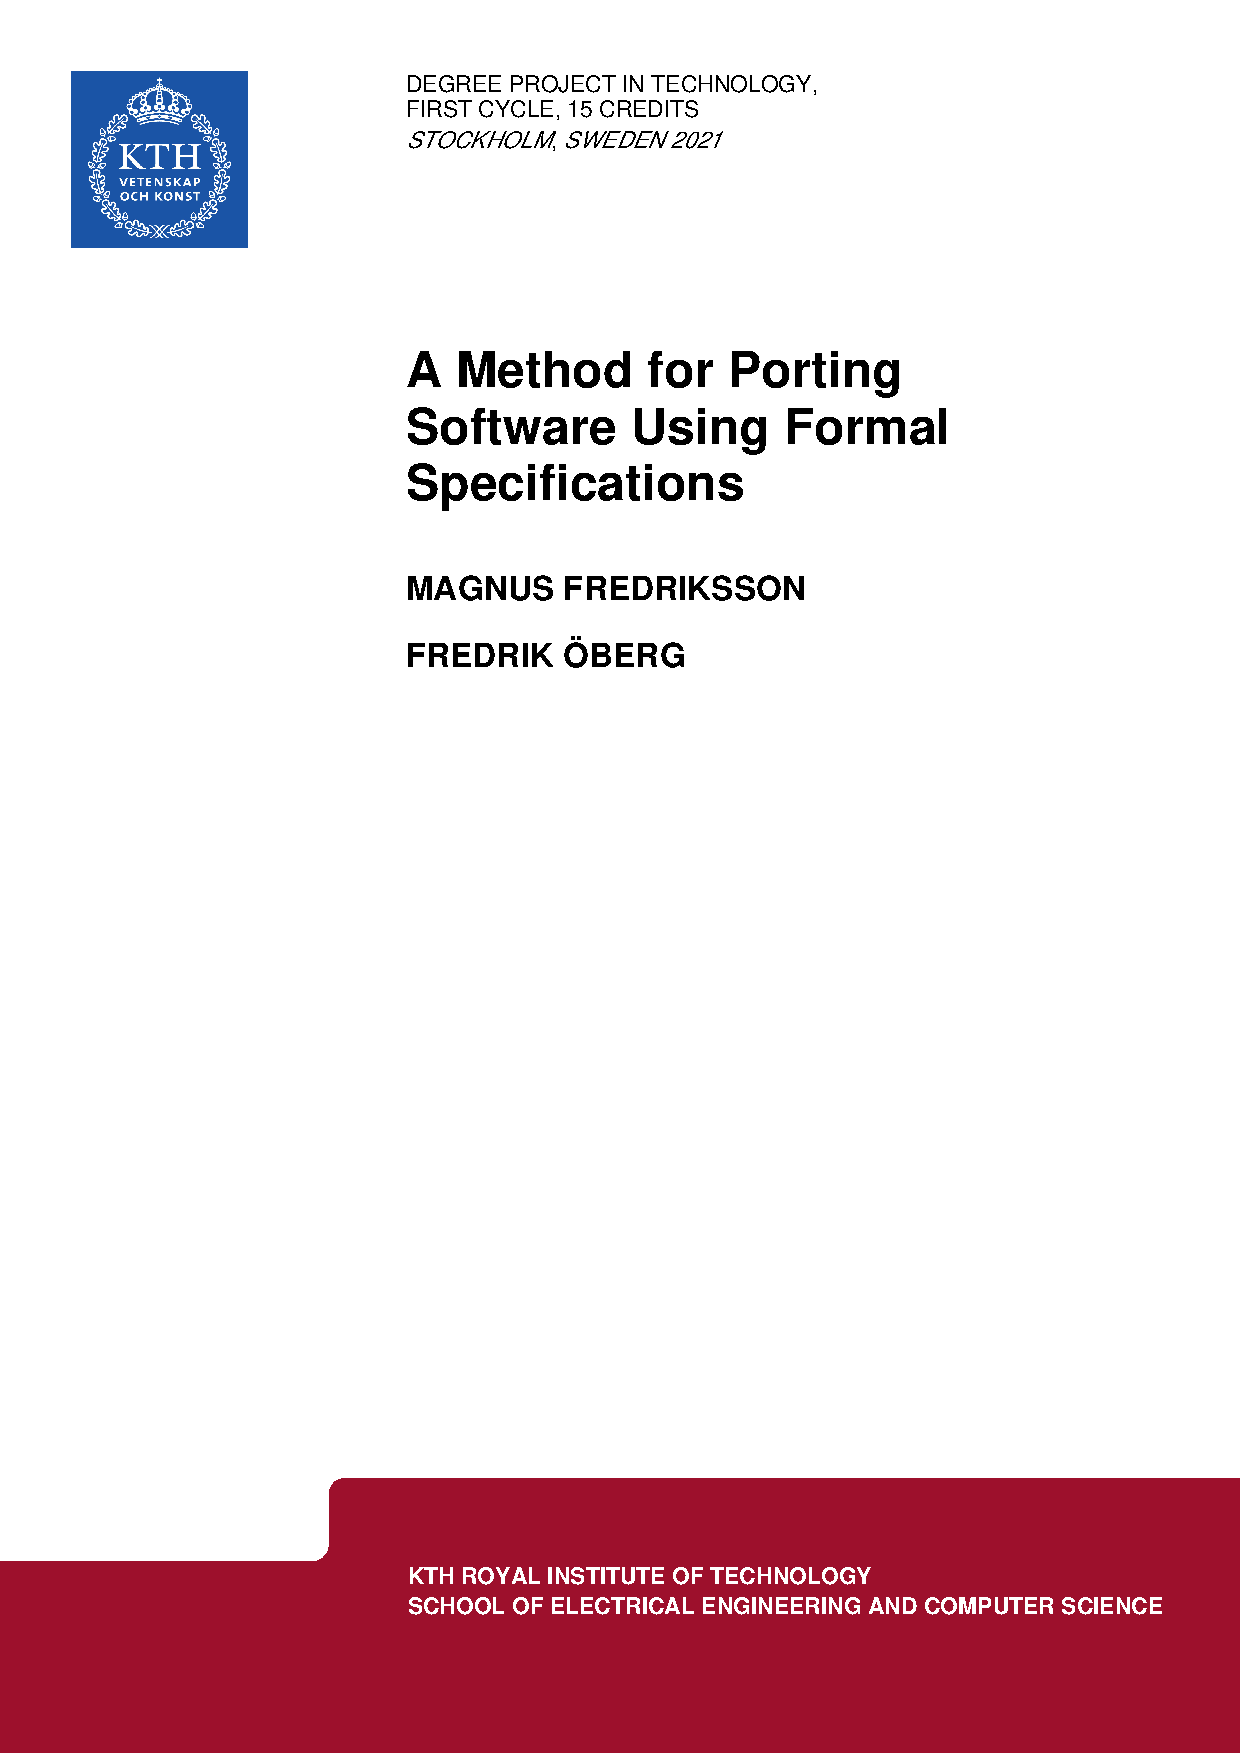
\includepdf[pages=-]{frontpage.pdf}




\hspace{0pt}
\vfill

\begin{abstract}

Formal specifications are mathematically based techniques with which a system can be analyzed, and its functionalities be described. Case studies have shown that using formal specifications can help reduce bugs and other inconsistencies when implementing a complex system; they are more likely found during the software design phase rather than later. 

During the process of porting code, testing has been used to verify that the port has the same functionalities as the original. However, testing alone has been deemed necessary but not sufficient to accomplish this. This thesis questions if formal specifications could be used during the process of porting code to create an accurate model of the system, and thereby provide higher degrees of certainty that the final product conforms to the original. 

A step-by-step methodology is presented to answer this question. The methodology ascertains the behavior of a port target through testing and a formal specification model based on these tests is created. This model is then used to create the port. The result indicates that the methodology used has some potential since it provided a high level of certainty that the ported code adhered to the original. Since the methodology puts a high emphasis on the specification and has several layers of verification, it is likely that it is suitable for projects with several modules and interdependencies. 

When using it for porting a trivial or non-complex system, the overhead of the methodology may prove high in comparison to the value gained. It was also found that one must take into consideration the implicit functionalities a language provides. Strict reliance on a model could thereby lead to a less flexible process where creativity and consideration of the specifics of the target language may have produced a different result.
 
\end{abstract}

\textbf{Keywords:} porting, formal specification, TLA+, testing, Rust

\vfill
\hspace{0pt}

\newpage
\selectlanguage{swedish}

\hspace{0pt}
\vfill

\begin{abstract}
Formella specifikationer är matematiska tekniker med vilka ett system kan analyseras och dess funktioner beskrivas. Fallstudier har visat att användning av formella specifikationer vid mjukvaruutveckling kan bidra till att reducera antalet fel och därmed minska omkostnaderna. 

Vid portering av kod har tester använts för att verifiera att porteringen har samma funktionaliteter som originalet. Tester anses dock vara otillräckliga - om än nödvändiga - för att fullständigt beskriva ett system. Denna avhandling ställer frågan om formella specifikationer kan användas i en porteringsprocess och därmed ge en högre grad av tillförlitlighet i att porteringen överensstämmer med originalet. 

En steg-för-steg-metodik presenteras för att besvara denna fråga. Metodiken använder sig av tester för att beskriva det system som skall porteras och en modell baserad på formella specifikationer skapas genom dessa tester. Denna modell används därefter för att skapa porteringen. Resultatet indikerar att metoden har viss potential eftersom den upplevdes öka förståelsen för referensarbetet och därmed också tryggheten i att den portade koden överensstämde med originalet. Eftersom metodiken lägger stor vikt vid specifikationen och består av flera lager av verifiering är det troligt att den är mer lämplig för system som består av flertalet moduler med inbördes beroende. 

Vid användning för att portera ett trivialt system kan metodens omkostnader visa sig vara för höga i förhållande till det värde som erhålls. Det visade sig även att en porteringsprocess måste ta hänsyn till de implicita funktioner ett språk tillhandahåller. En strikt anpassning till en modell kan därmed leda till en mindre flexibel process och därmed leda till ett icke tillfredsställande resultat, där kreativitet och hänsyn till målspråket skulle kunna ha gett ett annat.

\end{abstract}

\textbf{Nyckelord:} portering, formell specifikation, TLA+, testning, Rust


\vfill
\hspace{0pt}

\newpage
\selectlanguage{english}

\hspace{0pt}
\vspace{0.27\textheight}

 \section*{Acknowledgments }
  We would like to thank Rasmus Källqvist, Hind Kareem and Johan Montelius for their valuable input and continuous support during this project. 

\acknowlegmentssignature

\vfill
\hspace{0pt}




\setstretch{0.95}
\tableofcontents
\setstretch{1}
\newpage
\pagenumbering{arabic}
\section{Introduction}\label{introduction}

The computer software world is under constant development. New demands on a system could make it necessary to adapt it into a new environment than what it was originally designed for - a process called porting. 

\subsection{Background}

When porting software, one of the main concerns is that the functionality of the port adheres to the functionalities of the target source. The traditional way of verifying the behavior of computer software has been through the practice of testing. However, testing has limitations, and it is difficult to fully describe a system using testing alone \cite{testingisnecessary}. One way to complement the testing process to improve on this situation could be to set up a model of the system through a formal specification; a mathematically based technique with which the design of a system can be analyzed, and its functionalities be described with the purpose of helping with the implementation of systems and software. This means that independent of what language a software has been written in, if its behavior follows the formal specification, it provides functionality equivalent to any other software conforming to that same specification.

\subsection{Commissioned Work}
The customer for this project is Young Aces By Sylog (YABS); an IT consultant firm with one of its offices based in Stockholm, Sweden. As consultants they get hired to do work not normally part of their customers daily operations. A lot of this work concerns updating and porting system functionalities consisting of so-called legacy code. This is normally outdated code often severely limiting the performance of the system in question.

\subsection{Problem Specification}
The expressed problem that makes up the basis for this thesis is that the methods commonly used today are insufficient to verify the outcome of ported functionalities reliably. This thesis aims to answer the question: 

\textbf{is there a way to complement the current porting methods, which could increase the certainty that the ported code adheres to the original using a formal specification?}


\subsection{Purpose}

The use of formal specifications has indicated that it reduces the number of errors during software development. This practice has shown to create more reliable software while at the same time reducing production costs \cite{AMAZONFORMALSPEC}. The purpose of this thesis is to evaluate if formal specifications have the potential to provide a higher level of certainty that ported code adheres to the original. 

\subsection{Goal}
 
The goal of this thesis is to create a step-by-step methodology for porting software which uses a formal specification. Principally, to find whether the approach taken to incorporate a formal specification into the porting process yielded a valid result. A subjective evaluation of the strengths and weaknesses found when applying the methodology to the sample project will be made. 


\subsection{Target Audience}
The intended target audience is mainly practicing computer engineers as well as students of computer science interested in formal specifications and how it could be used in practice. It could also have the potential to be used as a basis for further work in the academic world.  

\subsection{Research Methodology}
The thesis will be performed as a qualitative case study where a detailed model for the methodology is described and then applied to a sample case. A method for evaluating the results will be described as part of the methodology and will be used to validate whether the process was successful. The quality of work and results of this thesis will be evaluated according to a set of quality criteria for qualitative research \cite{QUALITATIVE}.

\subsection{Delimitations}
The investigation's primary focus is on the feasibility of using formal specifications during a porting process; if it has the potential to be used to create a valid port of a system in a practical way by computer engineers during porting of computer software. The thesis will evaluate the validity of the port considering that the functionality provided is correct, but not whether it is achieved following any constraints on its performance.

The project is undertaken in a restricted time frame. Therefore, the scope of the source to which the methodology is applied is limited. This means that the efficiency of the method on other types of projects is left up to further investigation.


\section{Background}\label{background}

This chapter provides context to the information discussed throughout the thesis and is accomplished by providing theories, concepts, terms as well as historical data from relevant studies.

\textit{Verifying Programs Using Tests} describes two testing methods and some of their limitations as well as what a test-driven development (TDD) is. \textit{Verifying Programs Using Tests} also has a description of the concept of property-based testing. \textit{Formal Specification} provides a description of what the purpose of the technique is and how it has been used in the field of software development. It also contains a description of TLA+ which is the formal specification language used during this project. The sections \textit{C}, \textit{Rust} and \textit{Hoare Logic} provides background information about those topics and \textit{FreeBSD Linked List} describes the porting target source code and why it was chosen.






\subsection{Verifying Programs Using Tests}\label{testing}


Testing is, in general, performed in one of two ways. The first being where the functionality of the system is tested from an outside perspective without peering into its internal structure. This verifies that the expected outputs are produced on a given set of inputs and is a method usually called black-box, or functional testing. The second way of testing is where the internal structure and design of the program - its state - is being tested and is usually called white-box, or structural testing \cite{comparison}. It is not feasible through testing alone, by either of these disciplines, to guarantee the absence of bugs. It is only possible to verify that a piece of code behaves in some way given a specific, finite, set of inputs. Consider, for example, the pseudo-code in figure \ref{fig:pseudocode}.
\begin{figure}[H]
 \vspace{12pt}
\begin{verbatim}
                          
                          global signed z
                          function x(y):
                             z++           
                             y
                            
\end{verbatim}
    \caption{Pseudo-code Function}
    \label{fig:pseudocode}
\end{figure}

The function takes an argument as input and returns it without any mutation. It also applies the increment operator ++ on the global variable \textit{z}. As \textit{z} is signed, there are specific values of \textit{z} where the increment by one operator is not defined - namely the highest value that \textit{z} can take. From a black-box perspective, it could be concluded from even somewhat extensive testing, that the function behaves in a deterministic way and the rule described in figure \ref{fig:pseudoproperty} would hold.
\begin{figure}[H]
 \vspace{12pt}
\begin{verbatim}
                        [for all] numbers y     
                        x.apply(y) is y
                        
\end{verbatim}
    \caption{Pseudo-code Property}
    \label{fig:pseudoproperty}
\end{figure}

Achieving total coverage, even in this trivial example, would be time consuming since the input domain is all possible machine integers. It could also be the case that testing all of them would not necessarily find the bug since a possible undefined behavior of \textit{z} is independent of the functions input values. There are similar examples where the function would behave as intended when called in a certain application state, but potentially misbehave when the state is different, even if the input is the same each time. In the case of a more complex function which takes more input arguments making a linear search of the input space unfeasibly time-consuming. It could also be the case that even with many samples, the non-deterministic behavior of the function may not necessarily be exposed. Using metrics such as branches taken, or lines executed \cite{comparison} - common metrics for coverage - would not help in this case. 
Neither would automatically generate sets of input to be tested, so called property-based testing \cite{duregard_automating_2016}, necessarily find the problem since many consecutive calls to the function are needed (see section \ref{pbtesting}). The goal of testing thereby should be to find a reasonable set of tests that can verify the behavior for most input. They should also exercise the program's structural components thoroughly enough, no matter what is the correct, or intended behavior \cite{comparison}. 

By considering the structure of the program, it is possible to at least avoid constructing a set of tests which are guaranteed to be insufficient. The reasoning behind this is that it most certainly cannot be made any inference about the effects of a line of code if the line is never executed. Instead of doing an exhaustive search of the input space, structural tests give as good a guarantee that the code is covered, but with fewer test-cases. This is accomplished by basing the tests on the control structure of the program \cite{comparison} - in other words white-box testing. Tests written using the program's structural properties as a basis for test completeness should therefore be able to ascertain the behavior of the program to a degree sufficient for a starting point from which a mathematical description, or formal specification, can be created.

\subsubsection{Property-based Testing}\label{pbtesting}
Property-based testing is a way of using test-cases, not to check specific concrete cases, but rather as rules which describe some property of a function. The principle of property testing is described in \textit{QuickCheck} by K. Claessen and J. Hughes \cite{QUICKCHECK}. It entails that the test code describes some operation that is permissible unto the system under test along with the constraints on the input data for that operation. Along with the operation, some \textit{properties} such as pre- and post-conditions that must always hold true are defined. Usually this is done by the property function returning either true or false, or by using assertions. To then exercise this property, a set of concrete test-cases are automatically generated from this blue-print. The input data is usually generated according to some heuristic that is likely to find edge cases, e.g., "empty" style inputs, or inputs close to the perimeters of the range \cite{duregard_automating_2016}. This allows for a huge breadth of input parameters to be tested with very little effort.

There exists a subset of property-based testing, herein called stateful property-based testing. The purpose of this type of testing is to verify that properties of the system hold true, even over the lifetime of the system. To verify this, a model is defined. The model will usually be a simplified - but correct - version of the system under test (SUT). The model is used, before or after each operation, to verify some fact about the state of the SUT. For each operation on the SUT, a corresponding operation on the model is defined along with predicates that determine when the operation is valid. These operations can then be applied consecutively in different orders to find inconsistencies between the model and the SUT. Some testing frameworks will as an addition to finding the sequences of operations which yield inconsistencies, have some heuristic with which these sequences can be reduced to shorter ones \cite{QUICKCHECK}.

\subsubsection{Test Driven Development}

TDD is a common software development practice where tests are written first, and code is written only to satisfy these tests which initially should be failing \cite{TESTDRIVEN}. This leads to an incremental development process where development and testing is interleaved. One benefit to this process mentioned in \cite{sommerville_software_2011} is that it gives clarity to the intentions of the author - the tests make assumptions about how the code should behave explicitly. It is argued that because of this, tests make the code self-documenting. The fundamental process of TDD is an incremental, iterative one where implementation and refactoring is repeated until the tests pass \cite{sommerville_software_2011} (see figure \ref{fig:testdriven}).

\begin{figure}[H]
 \vspace{12pt}
\centerline{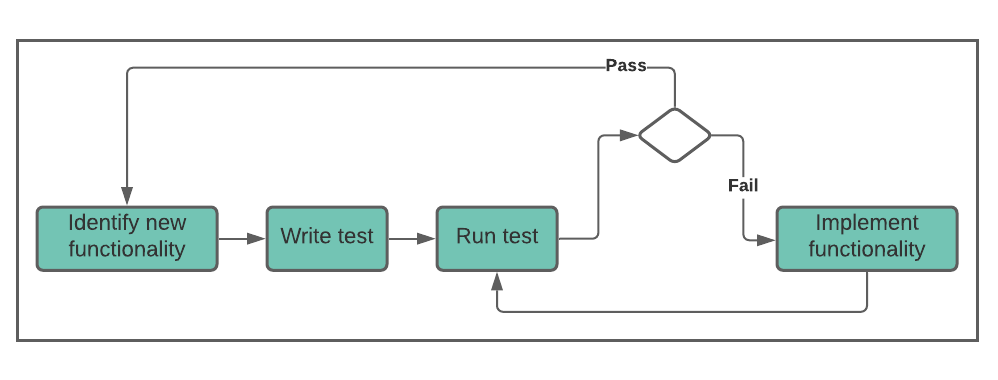
\includegraphics[width=4.8in]{TestDriven.png}}
\caption{The TDD Process}
\label{fig:testdriven}
\end{figure}

\subsection{Hoare Logic}\label{hoare}

Hoare logic is a formal system with a set of axioms and logical rules used in proofs of properties of computer programs \cite{HOARE}. Its central feature is the Hoare triple (see figure \ref{fig:hoaretriple}).

\begin{figure}[H]
 \vspace{12pt}
\begin{displaymath}
            P\{Q\}R   
\end{displaymath}
\caption{Hoare Triple}
\label{fig:hoaretriple}
\end{figure}

                        
This triple describes how the execution of a piece of code changes the state of the computation and should be interpreted as “if the assertion P is true before initiation of a program Q, then the assertion R will be true on its completion”. The use of this deductive reasoning is intended to provide a fundamental understanding of the code. 

\subsection{Formal Specification}\label{formalspec}


Building a software system is almost entirely a design activity consisting of combining, inventing, and planning the implementation of abstractions. The goal with this is to describe a set of modules interacting with one another in simple, well defined ways \cite{Larch}. If this goal is achieved it will enable engineers to work on different modules independently, while still accomplishing their common purpose. A good design will also make maintaining the software, as well as modifying its modules, easier without causing unintended effects. In summation, the key to good software design is inventing appropriate abstractions around which to structure the system.


Formal specifications are mathematically based techniques used to help with designing systems and software. Formal in this case means that they have a specific syntax, the domain of the semantics has a distinct set of meanings, and they can be used to infer useful information \cite{FORMALSPECROADMAP}. This enables them to demonstrate that a system is correct with respect to its specification while simultaneously describing system abstractions. This is accomplished independent of any of its implementations - specifications describe what a system should do, not how it should do it. This enables designers to focus attention on possible inconsistencies, deficiencies, and ambiguities leading to many mistakes and subtle bugs from many sources cropping up in specifications before they do in the implementation. This benefit could be derived from the fact that engineers focus on the safety and liveness properties of a system when using formal specifications; they need to state what needs to go right instead of focusing on what could go wrong, often a mind set when writing tests \cite{AMAZONFORMALSPEC}. Formal specifications encourage this way of thinking by describing an algorithm as a state machine, enabling a designer to create a simple and powerful abstraction of it.

\phantomsection
\label{benefits}
Since computer systems become increasingly more powerful and complex as time passes, the need for better techniques to assist in the design and implementation of reliable software becomes more prominent. Formal specifications have been around since the early days of computers and have been adopted in more traditional engineering disciplines but are not widely used in industrial software development \cite{sommerville_software_2011}. One of the reasons for this is that the method, by many, is not considered to be cost-effective. There has also been very little interaction between the test and formal specification communities, but some argue that the approaches could be used as complementary to each other for a better result \cite{USINGFORMALSPECTESTING}. 

Recent studies have also found that creating a mathematical model of a system under development led them to find and handle undesired behavior during the system analysis phase \cite{APPLYINGFORMALSPEC} \cite{AMAZONFORMALSPEC}. These studies claim that the time spent making mathematical models was well invested since it reduced the amount of time spent finding and fixing bugs during the implementation phase. This is most likely the case, since a model with good system-invariants helps engineers get the design right from the outset. The invariants capture the fundamental reason why the system works by using them as safety properties; properties that need to hold true for each possible state that the system can take. Therefore, they show that the design is not broken, which helps engineers get the code right faster since a broken design will lead to broken software - even if the code passes tests based on the design.
\\
\\
\\
Formal specifications due to its mathematical nature, however, are not an all-purpose tool. The consensus seems to be that they are most likely to be useful in data modeling where data definitions are written in a common, implementation-independent manner which lets the information pass through various development phases without transformation  This means that formal specifications are considered useful in situations such as when \cite{APPLYINGFORMALSPEC}:

\begin{itemize}
  \item There is a complex data structure that must be handled correctly.\label{formal_spec_structuer}
  \item A precise function definition is required when a simple function is needed, but it is vital that the function is implemented correctly.
  \item Complex functionality is involved with many choices to be made or many exceptional conditions arise.
\end{itemize}

To know when and how to use a formal specification takes a lot of skill and experience. For example, a formal specification does not easily model the performance of a system, and some aspects of performance cannot be modelled at all \cite{AMAZONFORMALSPEC}. If applied without consideration, a formal specification could therefore lead to a sub-optimal design even in the absence of errors. A feasible way to model a system to predict the issue of prolonged severe slowdowns seems to not be known as of this day \cite{AMAZONFORMALSPEC}. This means that other techniques need to be used combined with formal specifications to mitigate that. 

\subsubsection{TLA+}\label{tla}

TLA+ is a language developed by the computer scientist Leslie Lamport \cite{LAMPORTWEB} and has been used by, for example, Amazon since 2011 as a tool to achieve correctness in sophisticated distributed systems \cite{WHYAMAZONTLA}. They evaluated TLA+ among other languages like Alloy \cite{ALLOY} and Microsoft VCC \cite{MSVCC}. All languages had their pros and cons but TLA+ turned out to be best suited for their needs.

The evaluation found that TLA+ was best for handling very large, complex, as well as subtle problems. TLA+ was claimed to accomplish this by being able to capture rich concepts simply and directly without tedious workarounds, for example when specifying dynamic sequences of many types of nested records. It was also perceived that details from complex designs can be added or removed quickly since TLA+ supports arbitrarily complicated data structures with the ability to define powerful custom operators. This means that it was easy to adjust to a suitable level of abstraction making it a good tool when diagnosing bugs and subtle errors. Another property of TLA+ highlighted was that it tended to minimize the cognitive burden on engineers and accomplishes this by using conventional terminology since it largely consists of standard discrete math and a subset of linear temporal logic. This means that TLA+ allows for the expression of temporal relations between predicates, for example that some predicate will evaluate true \textit{eventually}, or that some predicate may be true only when another evaluates to some specific value. 

\subsubsection*{TLA+ Example}

A trivial example of how TLA+ can be used can be seen in this section, and is inspired by the works of Leslie Lamport \cite{LAMPORTVIDEO}.


\begin{figure}[H]
 \vspace{12pt}
\begin{verbatim}
                        global signed z
                        main()
                           z = someNumber()
                           z = z + 1
\end{verbatim}
    \caption{Program Example}
    \label{fig:programexample}
\end{figure}

The example program (see figure \ref{fig:programexample}) has an entry point \textit{main} and a global variable \textit{z} which gets assigned an integer through a call to the function \textit{someNumber}; a function returning said integer and has no side effects. The value of \textit{z} then gets incremented by one followed by the program terminating. This process can be described with a state machine (see figure \ref{fig:simplestatemachine}) which creates a simple abstraction of the code.

\begin{figure}[H]
 \vspace{12pt}
\centerline{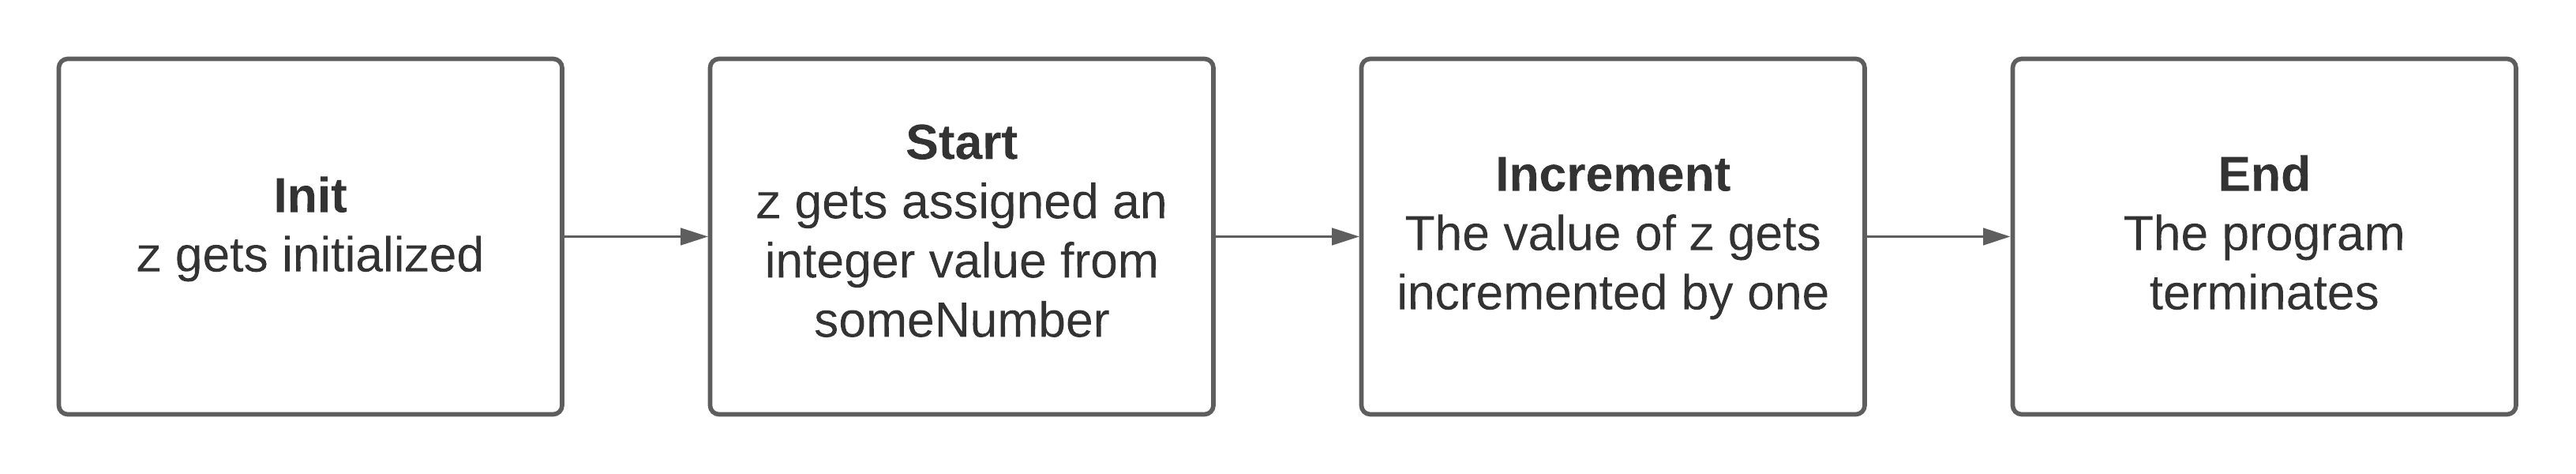
\includegraphics[width=5in, height=1in]{simplestatemachine.png}}
\caption{State Machine}
\label{fig:simplestatemachine}
\end{figure}

The state machine can then be implemented in TLA+ (see figure \ref{fig:tlaexample}). Here there is an additional variable defined called \textit{pc} which is short for program counter. It is used by the TLA+ model checker to know which state is the current one. The \textit{Init} label indicates the first state and initializes the value of the variables of the model, so the model checker knows where to begin. That the value of \textit{z} is initialized to 0 is a behavior of the language C and is used as an example but could differ depending on the language used when implementing the function. After the initializations, the model checker moves on to the label named \textit{Next} and checks which of the disjunctions (indicated by the or operator) holds true for every conjunction - in this case where the value of \textit{pc} is "start". \textit{z} then gets assigned its new value, indicated by the prime attached to it. It is accomplished by using the operator \textbackslash in which is equivalent to the mathematical operator $\in$ - member of. The function \textit{someNumber} is supposed to return any integer but TLA+ only allows for usage of finite sets. Therefore, as a compromise, \textit{z} is assigned an integer between 1 and 1000 indicated by the set operator ".." between those numbers. This means that \textit{z} becomes a member of the set of integers between one and one thousand in the current state. Lastly in this disjunction, \textit{pc} gets assigned its new value "increment". This means that the model checker moves to the state which holds true for the new value, checks it and proceeds with this practice until \textit{pc} is assigned the value “done” followed by its termination. This enables the model to be evaluated to see if every statement holds true given any situation, providing a logical foundation that the implementation does the same. If, however, it is not possible to satisfy one or more of the conjunctions, the model must be invalid, and cannot be implemented as an executable program.


\begin{figure}[H]
 \vspace{5pt}
\begin{lstlisting}
                VARIABLES z, pc

                Init == 
                    pc = "start" /\ z = 0
    
                Next == 
                    \/ /\ pc = "start"
                       /\ z' \in 1..1000
                       /\ pc' = "increment"
                    \/ /\ pc = "increment"
                       /\ z' = z + 1
                       /\ pc' = "done"
\end{lstlisting}
\caption{TLA+ Example}
\label{fig:tlaexample}
\end{figure}

\subsubsection*{TLA+ Tools}\label{tools}

The TLA+ ecosystem provides an integrated development environment (IDE) called TLA+ Toolbox \cite{TLATOOLBOX}, which allows for writing and translating the pseudo-code like language PlusCal into pure TLA+. PlusCal is a language that can express much of what TLA+ can express, but more conveniently. PlusCal even extends TLA+ with additional syntax and can be especially suitable for implementing algorithms \cite{PRACTICALTLA}.


\subsection{C}\label{c}

Since it started to gain popularity during the 1980s has the programming language C been a natural choice when programming at a low-level. Although C provides high level abstractions, nowadays C is considered a low level language due to the lack of automatic memory management and that it provides transparent, efficient access to the underlying hardware \cite{DEMYSTIFYING}. C found lasting use in applications previously coded in assembly. C provides many features not available in assembly such as several levels of scoping. This makes it possible to use the same identifier many times within a program without them necessarily interfering with each other. C also provides static type checking, meaning that type checking is performed at compile time. There are no strict rules about whether a language is strongly or weakly typed, however, since C allows the conversion of a void pointer to any other type and vice versa, it should not be considered strongly typed, Kernighan and Ritchie also consider it as such \cite{CPROGRAMMINGLANGUAGE}. 

One problem with C , especially nowadays when the alternative is not assembly language, but instead other modern programming languages, is the manual management of memory and the risks that come with this – a risk many would claim makes C an unsafe language \cite{RUSTONOMICON}. This comes from the fact that a misuse of manual memory management will cause undefined behavior. Bugs relating to mismanagement of memory can also be very hard to track down since such errors may lie dormant in the program until later when the program suddenly crashes or misbehaves. The program may also become unpredictable and create security vulnerabilities, for example when accessing some memory after the resource has already been freed (use-after-free) \cite{IMPACTOFUNDEFINED}. These problems among others have prompted the development of so-called safe languages \cite{JAVAWHITEPAPER}, many of which achieve safety through moving memory management into a layer not directly accessible to the programmer. This extra layer of virtualization - like most things - has an impact on the performance of the program often caused in large part by the garbage collector which must keep track of all allocated objects in real-time and reclaim them when they are no longer needed \cite{CPPJAVA}. 

\subsection{Rust}\label{rust}

Rust is a modern system programming language focusing on safety, speed, and concurrency and claims to accomplish these goals without using a garbage collector. Instead, the safety is enforced by the compiler by checking under what conditions objects in memory are being accessed or mutated according to some rules about data ownership. The rules regarding aliasing in Rust are quite strict, where aliasing means when two or more variables or pointers refer to the same or overlapping regions in memory. One of the most essential rules of Rust, regarding aliasing can be summarized as follows \cite{THERUSTPROGRAMMINGLANGUAGE}:

\textit{There may be one mutable \textbf{or} N number of immutable references to an object, but never \textbf{both} at the same time (N here could be any natural number).}

This is enforced statically by Rust's static analyzer called the borrow checker. The concept of mutability is also touched upon here, and it is important to understand that every variable or reference in Rust carries with it metadata about its mutability i.e. whether it can be modified. For example, if a stack-allocated variable like an integer is mutable, the programmer is allowed to reassign it with a new value. For references, mutability determines whether it is allowed to call the referenced object's mutable methods, change its properties directly, or pass it to a function that requires a mutable reference. 

By enforcing the rules at compile-time, rather than at run-time, code written in Rust can be as fast as code written in C. Designers of Rust also claim that introducing parallelism in Rust comes at a relatively low risk, since the compiler is designed to catch classical mistakes - such as race conditions - before execution \cite{RUSTONOMICON}. Code written in Rust is also claimed to always provide type- and memory-safety and situations like dangling pointers, use after free or any other kind of undefined behavior should never have to be endured by the programmer. This allows for more aggressive optimizations since they will not accidentally introduce crashes or vulnerabilities. The purpose of Rust is to eliminate the trade-offs that have been accepted when working with C while at the same time getting comparable performance \cite{THERUSTPROGRAMMINGLANGUAGE}.

\phantomsection
\label{safe}
Rust can be thought of as a combination of two programming languages - safe and unsafe Rust. Safe Rust is a subset of Rust and often considered the \textit{true} Rust programming language. This is where all the compile-time memory and type-safety checks are applied. Sometimes, however, there will be situations where low-level memory interaction is needed. In unsafe Rust, the programmer is allowed to dereference raw pointers and use other types of operations for which the compiler cannot provide the safety guarantees present in safe Rust \cite{THERUSTPROGRAMMINGLANGUAGE}. The value of this separation is that the programmer gains the benefits of having the option to use the benefits of an unsafe language — low level control over implementation details — without most of the problems that come with trying to integrate it with a completely different safe language \cite{RUSTONOMICON}. Another benefit to this separation is that the developer limits the number of lines of code that need to be debugged, whenever such a bug appears.


\newpage
\subsection{FreeBSD Linked List}\label{frebsd}


FreeBSD is a Unix-like operating system used to power modern servers and embedded platforms \cite{FREEBSD}. FreeBSD is mainly written in C, and its large codebase has been continually developed and updated since the beginning of the 90's by a large community of individuals and organizations. The codebase can therefore be considered well established and its functionality widely tried and tested. 

The LinkedList library in FreeBSD is defined in a queue header file, containing several function-like macros for a set of queue data structures. The singly linked list is a list where the ordering is upheld by the individual links themselves; each link - or node - defines the next element of the list, commonly using of pointers. To become useful in a computer program, each node in the list normally stores some value. In C this could be some structure or literal value, or a pointer to data somewhere else in memory.

\begin{figure}[H]
\centerline{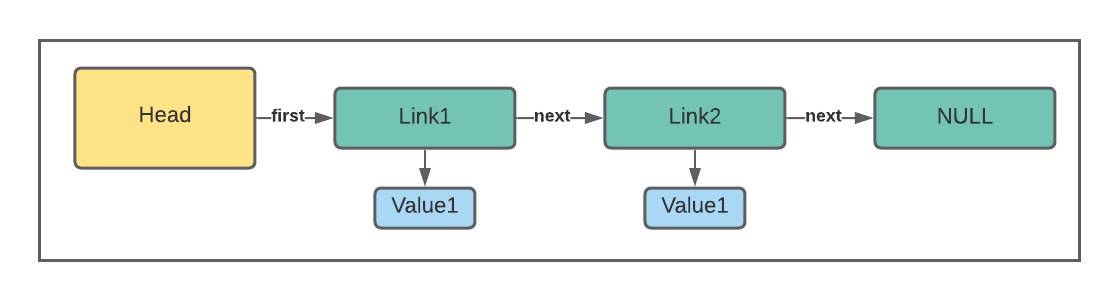
\includegraphics[width=5in]{LinkedList.png}}
\caption{FreeBSD Singly Linked List Structure}
\label{fig:freebsdlinkedlist}
\end{figure}

In the FreeBSD implementation of a singly linked list, the list consists of two structures: the head, which only contains a pointer to the first entry, and the node structure which contains some data and a pointer to the next node (see figure \ref{fig:freebsdlinkedlist}). 

\subsection{Summary}\label{motivation}

It has been shown that testing is a necessary part of software verification, but many times not sufficient for a complete understanding of a system. Property based tests with automatic test-case generation used in a white-box test discipline should maximize the utility of tests as a means of describing an existing system.

According to section \ref{formal_spec_structuer}, formal specifications can be considered most useful when handling a complex data structure. Although the complexity of a data structure is somewhat subjective, a linked list will likely contain enough complexity that the application of formalization provides some use. At the same it is common and straightforward enough that it should be understood easily by the target audience.

The properties brought up in this chapter made TLA+ a valid choice of language to use during this project. The argument is that TLA+ seems able to handle many types of problems as well as being easy be to learn. The available IDE with PlusCal support is another factor in the choice of modelling language.

If Rust manages to gain popularity and becomes ubiquitous, it is likely that it will be a target language for porting a large amount of C code in the future. Thus, the decision of using C and Rust as source and target language for this thesis seems, from the literature, as a valid and interesting choice. Using these languages will also hopefully help answering the question if formal specifications could help in getting a deeper understanding of the original system, as an intermediate step in the porting process. C and Rust, although meant to solve similar problems, have disparate design philosophies, and offer a differing feature set. This means that the linked list implementations have the potential to look vastly different. A model can describe the system without using language specific constructs, which will be important in bridging the differences of the languages.

The FreeBSD list library includes several different queues and lists. Of these, the singly linked list was chosen as the sample to port. It should to the target audience be a familiar data structure, and it is one with which the authors are well versed. Choosing a common data structure as the subject should reduce the amount of time needed to understand and describe its intricacies in greater detail.


\section{Method}\label{method}
This chapter provides a clear and extensive description of the methodology undertaken to address the question the thesis is based on. The intention is to enable the methodology to be reproducible. This is accomplished by dividing the method into several steps and for each one describing the processes they involve, the tools used, and criteria for completion.
 
\subsection{Structure}\label{structure}

To answer the question if formal specifications can be used during porting processes, the methodology was divided into discrete steps (see figure \ref{fig:vmodel}).
The steps and their ordering can be compared to the V-model; a widely adopted software development project model \cite{VEEMODEL}. The V-model describes a procedure, where high-level requirements are assembled first and then as the process goes on, the detail level is increased until implementation. The model also describes verification stages corresponding to each of these previous stages. The verification begins with the smallest granularity of tests and becomes more high-level until finally acceptance testing is performed. The methodology described in this thesis, can be seen as an inversion of the V-model where the process starts already having an original source. By writing tests, the behavior of the original was ascertained. On the highest abstraction level, the model specification lives. This represents the high-level requirements of the traditional V-model. The last verification step exists as a bridge between the original source and the ported source. Figure \ref{fig:vmodel} shows a minimal representation of the V-model, and how this process can be seen as an inversion of it.   

\begin{figure}[H]
\centerline{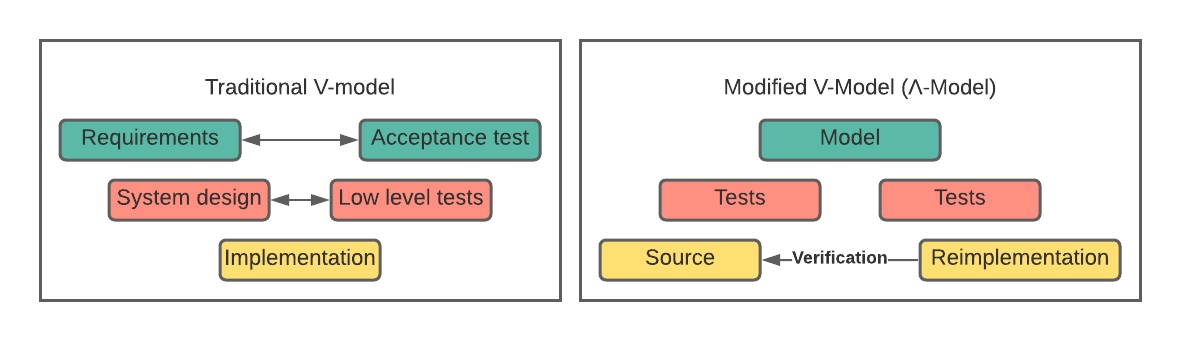
\includegraphics[width=5in]{V-model_.png}}
\caption{Simplified V-model of Software Development, Alongside a Modified Version of the Model}
\label{fig:vmodel}
\end{figure}
\newpage
To get a more detailed description of the method, it was divided into the following steps: 

\begin{enumerate}
  \item Find an established and well used open-source library as a target source code.
  \item Select a suitable testing framework and implement tests on the target source code to form an understanding of its behaviors and functionalities.
  \item Find a formal specification language and reverse engineer the target source code by creating a model of it. This model is to be derived from the tests implemented in the previous step.
  \item Implement tests for the functionalities specified in the created model.
  \item Implement the functionalities in the target language based on the tests created.
  \item Verify that the implementation is a true port of the target source code using a verification test-suite. The test-suite should run on both the original compiled code and a compiled version of the new implementation without modification.
\end{enumerate}



\subsection{Testing}\label{tests}

For this thesis, testing was performed to create an understanding of the system under test. This is a reversal of the traditional role of the test code. To select tools and metrics that fitted this purpose best, constraints that applied to this specific scenario were considered. The tests needed to be able to verify to such a degree that all the behaviors of the code were accounted for. For example, there could have been some scenario which yielded unintuitive results; some behavior that did not match the porting parties' expectations. It was important to find these cases, not to expose them to fix, but to build a complete understanding of what the code did. 

To achieve this in as an efficient manner as possible, the test-methodology chosen for the thesis fell on property-based testing. This practice entails that the test code describes some operation that is permissible to the system under test along with the constraints on the input data for that operation (see section \ref{pbtesting}). This approach was assumed to be particularly useful for this endeavor because it can be utilized without knowing the intentions of the system under test and can be seen as a guided exploration on the test subject rather than verification.

Like most data structures, the subject of the port will likely have some state which may or may not be permuted by the available operations. To make sure that the tests fully exercise this property of the code, and that the assumptions made also hold true over the lifetime of the system, a stateful test-suite was also created (see section \ref{pbtesting}). This meant that some operations and predicates which determine when the operation is valid were defined, along with a model. 

To perform all these tests, a test framework was used. A test-framework provides a convenience in the test-writing process, foremost since it provides some code to drive the tests - code often referred to as a test runner. This frees the developer from the burden of verifying that all tests are run, as well as collecting statistics and logging failures. To determine when tests were sufficient, the metric of test-coverage by branch and line-of-code was used. That way it was easy to verify that each branch, and/or line had been exercised. There were, therefore, some requirements that a chosen framework had to fulfill to satisfy the needs of the project.

\subsubsection{Frameworks}

The choice of frameworks fell on GoogleTest \cite{GOOGLETEST} as it was a widely adopted unit testing library. It also allowed tests to be written in C++ which enabled the subject to be easily tested with minimal modification. RapidCheck \cite{RAPIDCHECK} was chosen as a framework for the property-based testing since it was easy to use alongside GoogleTest; RapidCheck allows for specification of properties in an imperative style which works well for C++. 


\subsubsection{Environment}\label{environment}

To execute tests on the C source code, a test environment needed to be set up. The project and dependencies were acquired and built automatically using CMake \cite{CMAKE} which is an easy-to-use tool for automating these types of procedures. As an IDE, CLion \cite{CLION} was chosen as it is a cross-platform IDE for C and C++. CLion also provides integration with CMake, allowing for a simple build procedure. The GNU C++ compiler g++ was used to compile the source code \cite{GCC}.

\newpage

\subsubsection{Implementation Process}\label{implproc}

The initial intention was to create tests in a methodical and structured way. To accomplish this, these steps of deductive reasoning and test implementations, inspired by Hoare logic (see section \ref{hoare}), were created and followed:

\begin{enumerate}
  \item Select a functionality to write tests for.
  \item Provide a logical basis for the program properties. This should be done by making several assertions on the functions precondition as well as on the results obtained on termination i.e., the values which the relevant variables will take before and after execution of the program. 
  \item Create tests based on the logical basis to see if the program is understood correctly and carries out the functionalities identified.
  \item Modify tests to match any discrepancies found between actual and expected behavior.
  \item Repeat all steps until all functionality of importance has been identified and tested.
\end{enumerate}


\subsection{Reimplementation}\label{reimpl}
A TDD methodology was the approach chosen when implementing the formal model into Rust code, interleaving writing the tests with the actual implementation. The TDD used in this project followed the steps defined in figure \ref{fig:testdriven}, with the addition that new functionalities are found only from the model, by one of its invariants. The tests should be written so that when they pass, an invariant - or part of one - should be fulfilled. The fact that the tests are based on the model - and TDD's self-documenting nature - should make explicit the relation between the model and the implementation.

\subsection{Verification}\label{verification}

With the ported code in place, it should behave the same way as the original. To verify this, the port and source were both built as linkable libraries sharing the same application programming interface (API) allowing them to be tested by one single set of tests (see figure \ref{fig:api}). This made it possible to swap out the system-under-test without changing the test-code, thereby serving as an independent verification that the two implementations behaves the same. This can be compared to how hardware components can be tested in a single test-bed and quickly swapped out for the next component.

This verification process requires that the source and target language have interoperability with, and can be called by some common language, preferably the one used to write the original tests (see section \ref{implproc}). In the case of this project - where C and Rust were the languages used - interoperability can be achieved by creating a foreign function interface (FFI) by declaring matching external functions that call the appropriate library functions. 

\begin{figure}[H]
\centerline{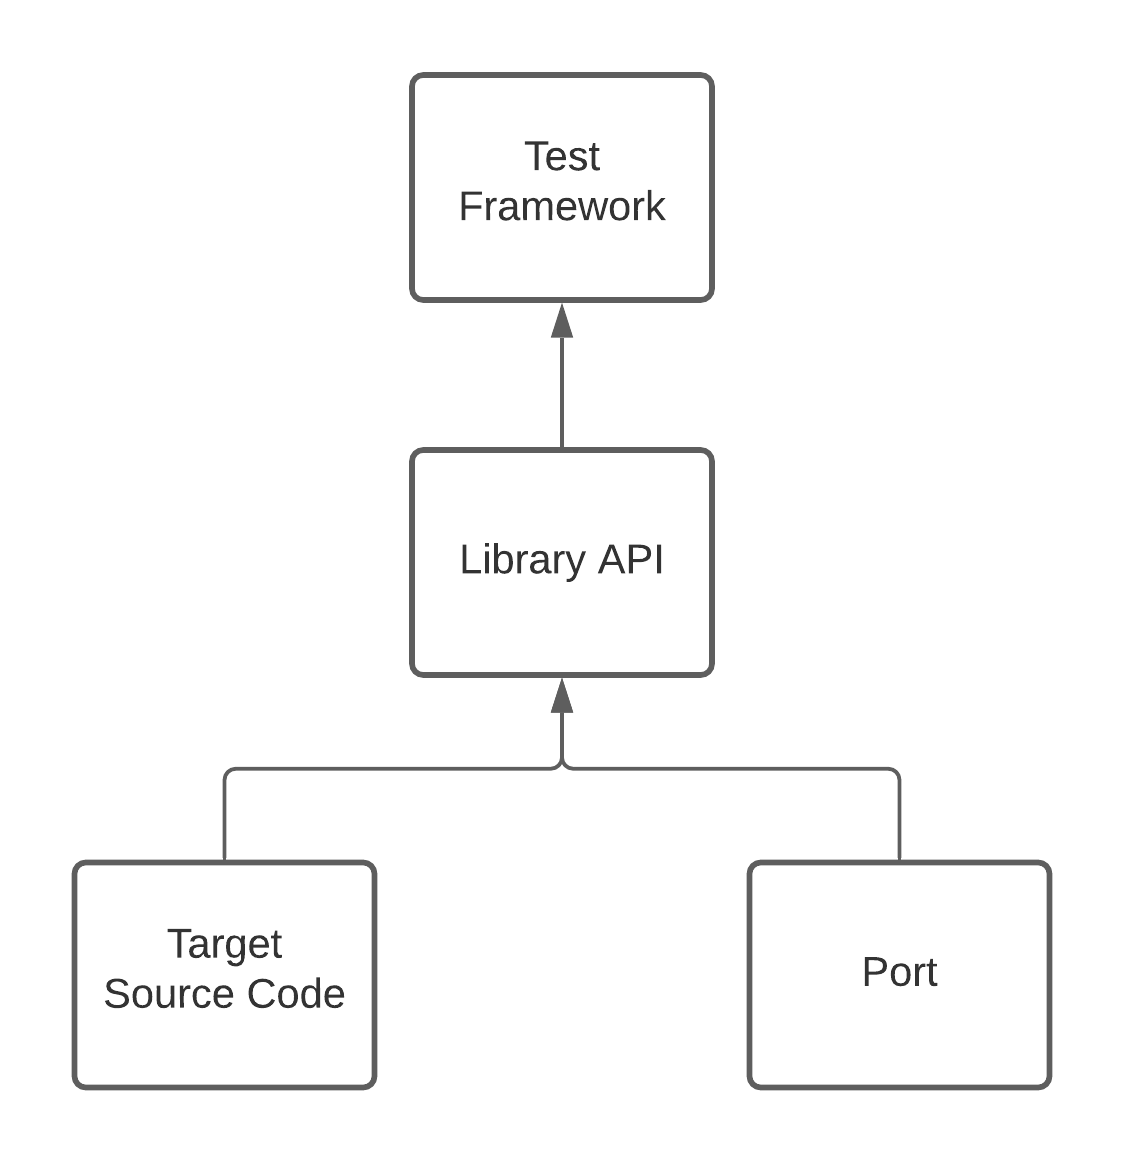
\includegraphics[width=2.5in]{api.png}}
\caption{Verification Structure}
\label{fig:api}
\end{figure}

As well as serving as the final evaluation of the final product, whether this last step is successful also serves as an evaluation of the method proposed. If it is successful then it can be concluded that this method is a feasible way of porting software. There is one caveat to this last step of the method process, knowing some of the differences between C and Rust. While the intention is to leave the original library as unmodified as possible, it may be necessary - or at least convenient - to insert one or a few helper functions into the library version of the source that manages the creation of lists etc. This will likely aid in keeping the interfaces to the libraries identical, while allowing the ported code to be more Rust “idiomatic”. The key to the success of this type of verification process will be to not add functionality influencing the test results, and consequently invalidating the conclusion of the tests.

\section{Implementation}\label{result}

This chapter serves as a documentation of the resulting code when following the porting methodology specified in the previous chapter. This is accomplished by showing the step-by-step process of how the porting of a function was accomplished. The functionality chosen as an example throughout this chapter is the concatenation of two separate lists into one. For each step in the process a sample implementation of the concatenation operator is presented. This choice was made since it is one of the less trivial functions of the original C code, providing a better foundation for the reader to get a grasp of how the porting process was applied. The complete implementation result can be seen at the project's GitHub repository \cite{LINKEDLISTREPO}.

\subsection{Environment}

The first step in the process was to isolate the files needed by the data structure so that they could be executed outside the context of the FreeBSD codebase. As the linked list code chosen was in the lower levels of the operating system, this was an elementary process since there few dependencies needed to be included. However, some FreeBSD specific OS-level definitions which were not present in the Linux standard library needed to be included. This complicated the process somewhat but was solved by including these into the queue source.

The linked list source code was fully made up of macros; predefined text snippets that are expanded into code during the pre-processing stage of compilation. This meant that the macros needed to be expanded into valid C code so that coverage of any tests could be measured. This was done by using the GCC compiler and the -E flag \cite{gcc_man}. However, using this method when expanding code directly would yield no output since macros are expanded where they are used, not where they are defined. Therefore, a level of indirection was added by defining proxy functions using the macros which as well as expanding the text into valid C code enabled the coverage of this code to be measured. The added indirection somewhat changed the semantics of how the library was invoked by introducing function calls that would otherwise not be present. Defining these functions as inline could make it so that the resulting compiler output was identical, or very close to the one generated using the macros directly.
    

\subsection{Behavioral Properties}

The source code of the concatenation function (see figure \ref{fig:concat}) shows that the function takes two lists as arguments named \textit{head1} and \textit{head2} (line 2 and 3). The argument names come from the fact that the first node of a list is referred to and stored in a head structure but will, where appropriate, be referred to as lists. The function concatenates the two lists into one where the head of the first list becomes the head of the concatenated, and the second lists head is set to be the next element to the tail of the first list. This indicates that the tail of the second list becomes the tail of the concatenated list.
\begin{figure}[H]
 \vspace{12pt}
\begin{lstlisting}[style=CSTYLE, belowskip=1pt]
void SLIST_CONCAT_impl(
    mySinglyLinkedListHead* head1, 
    mySinglyLinkedListHead* head2){
    IntegerSLISTEntry *curelm = head1->slh_first;
    if (curelm == NULL) {                                    
        if ((head1->slh_first = head2->slh_first) != NULL) {
            head2->slh_first = NULL;                                   
        }
    } else if (head2->slh_first != NULL) {               
        while (curelm->entries.sle_next != NULL){  
            curelm = curelm->entries.sle_next;         
        }                                                                                                              
        curelm->entries.sle_next = head2->slh_first
        head2->slh_first = NULL
    }
}
\end{lstlisting}
    \caption{The Concatenate Function}
    \label{fig:concat}
\end{figure}
The concatenation is accomplished by first checking if the first list - the \textit{head1} pointer argument - is populated by any nodes (line 5). If that is the case, it assigns the head of the second list, the \textit{head2} pointer argument, to the address of the first. This is done while in the same statement checking if the second list is populated (line 6). If it is, it sets the second list to be empty to avoid duplicate references (line 7). 
In the case of the first list being populated, the function checks in the else if clause if the second list is populated as well (line 9). If it is, then the function iterates through the first list to reach its tail element (lines 10 to 12). The head of the second list then becomes the next element of the tail element in the first list (line 13). This makes the second list appended to the first i.e., they are now concatenated. As a last statement is the head of the second list set to NULL (line 14). This shows that the function not only "copies" \textit{head2} onto \textit{head1}, but "moves" the second list onto the end of the first.

When describing the valid states and functions of the program, a hypothesis about a certain function was deduced from the code using the previously mentioned Hoare logic (see section \ref{implproc}). This means that for each function of the target source code were a set of pre- and post-conditions identified. Each precondition needed to identify valid initial states on which the function could be applied, and each post-condition needed to be a statement about the resulting state of the list that should be true after the execution of the function. To form a behavioral understanding on the preconditions of the concatenate function, it can be stated that the function takes two lists as arguments. This allows the conclusion that the precondition can be based on the following four situations:

\begin{itemize}
  \item Both lists are empty
  \item The first list is populated and the second is empty
  \item The first list is empty and the second is populated
  \item Both lists are populated
\end{itemize}

These four situations form the foundation for these following behavioral statements where the first one is when both lists are empty. In \ref{fig:prop1} and forward, the list variables are prepended with P or R - corresponding to the Hoare logic (see section \ref{implproc}) - indicating whether they are the values before or after the operation (see figure \ref{fig:prop1}). The \textit{isEmpty} helper function indicates whether a list is empty, and the behavioral reasoning states that if both lists are empty, the test needs to check that both lists still are empty after the concatenation procedure. 

\begin{figure}[H]
 \vspace{12pt}
\begin{verbatim}
       Precondition: isEmpty(P_list1) AND isEmpty(P_list2)
    
       Function: concatenate(P_list1, P_list2)
    
       Postcondition: isEmpty(R_list1) AND isEmpty(R_list2)
\end{verbatim}
    \caption{Properties of Concatenation Operation 1}
    \label{fig:prop1}
\end{figure}


Following this stipulation, it can be stated that the two cases where only one list is populated results in the same end state. This forms the behavioral basis seen in figure \ref{fig:prop2}. The \textit{validList} helper function checks that a list is valid, \textit{size} returns the number of elements in the list and \textit{first} and \textit{last} return the first and the last element of a list.

\begin{figure}[H]
\begin{verbatim}
       Precondition: 
           • case1 -> validList(P_list1) AND isEmpty(P_list2)
           • case2 -> isEmpty(P_list1) AND validList(P_list2)
        
       Function: concatenate(P_list1, P_list2)
    
       Postcondition:
           • case1 -> isEmpty(R_list2) AND
                      first(R_list1) = first(P_list1) AND
                      last(R_list1) = last(P_list1) AND 
                      size(R_list1) = size(P_list1)
           • case2 -> isEmpty(R_list2) AND
                      first(R_list1) = first(P_list2) AND
                      last(R_list1) = last(P_list2) AND
                      size(R_list1) = size(P_list2)
\end{verbatim}
    \caption{Properties of Concatenation Operation 2}
    \label{fig:prop2}
\end{figure}


This basis indicates that the tests need to assert that the head of the first element of the populated list in the precondition always is returned being assigned to the element of the first list in the post-condition. It must as well assert that the last element of the populated list becomes the last element of the concatenated list. The tests must also assert that the second list in the post-condition always is empty, and that the length of the concatenated list always is of the same length as the initially populated one. 

If both lists are populated the behavioral basis becomes more complicated since several more assertions can be made on the post-condition (see figure \ref{fig:prop3}). 
\begin{figure}[H]
\begin{nonbreaking}
\begin{verbatim}
       Precondition: validlist(P_list1) AND validList(P_list2)
    
       Function: concatenate(P_list1, P_list2)
    
       Postcondition: first(R_list1) = first(P_list1) AND
                      last(R_list1) = last(P_list2) AND
                      size(R_list1) = 
                      (size(P_list1)+size(P_list2)) AND
                      isEmpty(R_list2) AND
                      {P_list1} SUBSETOF {R_list1} AND 
                      {P_list2} SUBSETOF {R_list1}
     
\end{verbatim}
\end{nonbreaking}
    \caption{Properties of Concatenation Operation 3}
    \label{fig:prop3}
\end{figure}


This behavioral basis states that in the case of both lists being populated, the head of the concatenated list must always be the head of the first list in the precondition. The basis also indicates that the tail of the second list always becomes the tail of the concatenated list. Since the lists are being concatenated the size of the concatenated list must also always match the sum of the size of both initial lists. This also means that the size of the second list always must be zero as a post condition i.e., the second list becomes empty. Lastly it states that the nodes of the two initial lists must always be a subset of the concatenated list.

\subsection{Tests}

To verify that the actual behavior conformed to the behavioral basis, tests were written asserting that this is the case. Both unit and stateful property-based tests were written in \textit{GoogleTest} combined with \textit{RapidCheck}. An example of a testing property for the concatenate function takes vectors of integer values (see lines 3 and 4 figure \ref{fig:size}) generated by \textit{RapidCheck} and converts them into two separate lists of the \textit{mySinglyLinkedList} type through the helper function \textit{createList} (lines 6 through 9). These vectors were of an arbitrary number of elements, including empty. 

\begin{figure}[H]
 \vspace{12pt}
\begin{lstlisting}[style=CSTYLE] 
RC_GTEST_PROP(SLIST, 
concatenatingListsYieldsCorrectSizeOnList1, 
(std::vector<IntegerSLISTEntry> a,
std::vector<IntegerSLISTEntry> b)){

    mySinglyLinkedListHead headA{nullptr};
    createList(headA, a);
    mySinglyLinkedListHead headB{nullptr};
    createList(headB, b);
    unsigned int expectedSize = a.size() + b.size();
    
    SLIST_CONCAT_impl(&headA, &headB);
    
    IntegerSLISTEntry *entry;
    int actualSize = 0;
    
    SLIST_FOREACH(entry, &headA, entries) {
        actualSize++;
    }
    
    RC_ASSERT(expectedSize == actualSize)  
    RC_ASSERT(headB.slh_first == nullptr);
}
\end{lstlisting}
    \caption{Size Test}
    \label{fig:size}
\end{figure}
After the lists have been concatenated the test asserts that the size of the concatenated list always is of the same size as the sum of the sizes of the two separate lists (see line 21 figure \ref{fig:size}). This is enabled by saving the total size of the two vector arguments in the variable \textit{expectedSize} (line 10). This variable is then compared with the variable \textit{actualSize} which receives the size of the concatenated list by iterating through every element via the target source code macro function SLIST\_FOREACH which increments \textit{actualSize} by one for each iteration (lines 17 and 18). The test also asserts that the second list is always empty after the concatenation procedure (line 22). These procedures provide verification coverage that the size state of the lists found during the behavioral understanding stage (see section \ref{implproc}) holds for every tested situation.
\begin{figure}[H]
 \vspace{12pt}
\begin{lstlisting}[style=CSTYLE]
struct SLIST_concatenate : 
    rc::state::Command<SLIST_model, mySinglyLinkedListHead> {
    
    std::vector<int> concatenate_with = 
        *rc::gen::arbitrary<std::vector<int>>();

    void apply(SLIST_model &model) const override {
        for(auto i: concatenate_with)
        model.list.push_back(i);
    }

    void run(
        const SLIST_model &model, 
        mySinglyLinkedListHead &head1) const override {
        auto head2 = new mySinglyLinkedListHead();
        createList(head2, concatenate_with);
        SLIST_CONCAT_impl(&head1, head2);
        RC_ASSERT(SLIST_EMPTY_impl(head2));
    }

    void show(std::ostream &os) const override {
        os << "SLIST_CONCAT: ";
        for(auto i: concatenate_with) { os << i << ", "; }
    }
};
\end{lstlisting}
    \caption{Stateful RapidCheck Test Structure}
    \label{fig:statefulrc}
\end{figure}

Along with the unit-test style cases, a property-based stateful test-suite was created for the list type. Stateful meaning that each test is executed on the same or equivalent instance of the system-under-test, and any mutation to the system is retained for the next operation. To verify the state at each point, a model was inserted into the test suite. This model is some simplified version of the system under test that implements equivalent operations, and with which the system state is be verified to be correct. In this test-discipline, a set of operations were defined. Each operation implements a function that mutates the model, and one that mutates the system-under-test as well as optionally any assertions that can be made to verify that the system state conforms to the model state. The operations also optionally define some constraint under which it is valid. This allows for operations to be skipped when the operation is not properly defined for the current model state, e.g., getting the first element of an empty list. Operations were defined by implementing a class (see figure \ref{fig:statefulrc}). In the case of the concatenate operation, an arbitrary vector was generated to create a list (lines 4 and 5), used as the basis for the concatenation (lines 14-18).

To verify that all branches of the tested code were covered by the tests, coverage metrics were collected using the tool gcov and visualized with lcov (see figure \ref{fig:lcov}). This allows for metrics such as which branches were not executed, and how many times each line was executed to be easily ascertained. After the tests specified by the behavioral bases were implemented, the coverage was checked to make sure no lines or branches were untested.

\begin{figure}[H]
\centerline{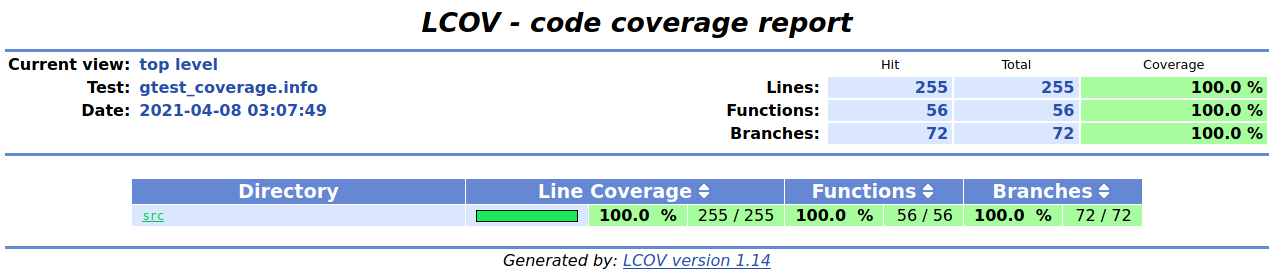
\includegraphics[width=5in]{lcov_ui.png}}
\centerline{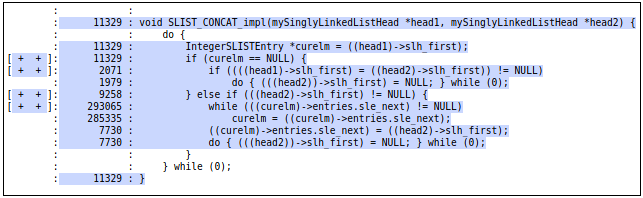
\includegraphics[width=5in]{lcov.png}}
\caption{Visualization of Coverage Metrics Using lcov}
\label{fig:lcov}
\end{figure}

\subsection{Model}

With the tests in place, it was time for the creation of the TLA+ model. The model was split into two modules named LinkedList and Main. LinkedList describes the data structure itself, the structure of the data and the operations that are permitted to be performed on it. Main contains the model checking algorithm verifying that the model works for each possible state,  as well as the invariants verifying that the structure of the linked list holds for each state of the algorithm.

TLA+ almost entirely consists of mathematical sets and functions. Therefore, inspired by the linked list implementation in the book Practical TLA+ \cite{PRACTICALTLA}, was the linked list in this implementation defined as a function. It has a domain of a set of labels, which could be a pointer or a reference in a source code implementation, where each domain entry represents a node in the linked list. The range of the function consists of a function with a finite domain with the labels next and value representing the variables stored in each node (see figure \ref{fig:linkedlists}). 


\begin{figure}[H]
 \vspace{12pt}
\begin{verbatim}
          [NULL |-> [next |-> NULL, value |-> NULL]]
        
          [label1 |-> [next |-> NULL, value |-> INT], 
           label2 |-> [next |-> label1, value |-> INT],
           label3 |-> [next |-> label2, value |-> INT]]
\end{verbatim}
    \centering
    \caption{Linked List Examples}
    \label{fig:linkedlists}
\end{figure}


The label “next” maps to some other label in the linked list domain, indicating that it is the element following the current of the list, or NULL, indicating that the current node is the last. The “value” label maps to some integer held by each node, which in the target source code could be any arbitrary primitive data type or structure.

To check that a function is a valid linked list, a TLA+ operator called IsLinkedList was created (see figure \ref{fig:islinkedlist}). It takes a function as argument, named PointerMap, and checks that for each element in the domain of the PointerMap - NULL included and the label of the first element of the list excluded - there exists a node with the next value representing each node in the function. If that is the case it returns true and false if not. Based on this definition, lists containing cycles are also excluded.

\begin{figure}[H]
 \vspace{12pt}
\begin{verbatim}
        IsLinkedList(PointerMap) ==
            \A el \in ((DOMAIN PointerMap \union {NULL}) \ 
            {First(PointerMap)}): \E x \in DOMAIN PointerMap:
            PointerMap[x]["next"] = el  /\ el /= x
\end{verbatim}
    
    \caption{IsLinkedList Operator}
    \label{fig:islinkedlist}
\end{figure}


As a part of creating arbitrary lists for usage during the model checking process, an operator called PointerMaps was created. It creates a set of functions by mapping from a domain of unique labels it receives as argument to a range (see figure \ref{fig:pointermaps}). PointerMaps creates with this every possible permutation of the domain mapping to every possible permutation of the next range. This means that PointerMaps creates a set of functions that include all valid lists, but also mappings which are not valid.

\begin{figure}[H]
\vspace{12pt}
\begin{verbatim}
    PointerMaps(domain) == 
        [domain -> [value: VALUE, next: domain \union {NULL}]]
\end{verbatim}
    \caption{PointerMaps Operator}
    \label{fig:pointermaps}
\end{figure}


PointerMaps, in combination with IslinkedList, is used in an operator called LinkedList which filters the output from PointerMaps by choosing one of the mappings that IsLinkedList validates as a LinkedList (see figure \ref{fig:linkedlist}). This list, represented as the variable pm, is then returned to be used in the model checking algorithm. If LinkedList on the other hand receives an empty set of domain labels, it returns the representation of an empty list. The empty list is a special case, where NULL is allowed as the only value in the domain of the list (see figure \ref{fig:linkedlists}).

\begin{figure}[H]
\begin{verbatim}
      LinkedList(domain) == 
          IF NULL \in domain 
              THEN Assert(FALSE, "Null cannot be in domain") 
          ELSE IF domain \subseteq {}
              THEN EmptyList
          ELSE
              CHOOSE pm \in PointerMaps(domain):
              IsLinkedList(pm)
\end{verbatim}
    \caption{LinkedList Operator}
    \label{fig:linkedlist}
\end{figure}


With the definition and the ability to create linked lists in place, the concatenation function was added to the model (see figure \ref{fig:concatenation}). It was accomplished via a TLA+ operator taking two lists as arguments and checks if either of the lists are empty. If that is the case, it returns the lists in a TLA+ sequence specified with $<$$<$ $>$$>$, where the empty list is placed at the second index of the sequence. A TLA+ sequence is another way of representing a function where the index of the sequence is equivalent to the domain of a function. It is used in this case to enable the operator to return two lists in a specified order to enable usage using the model checking process (see figure \ref{fig:pluscalconcat}). If both lists are populated there is the special situation where the next value of the last element of the first list needs to be mutated. This is needed since the last element of a list always points to a NULL value and instead needs to show the label of the first element in the second list for them to be considered concatenated.

\begin{figure}[H]
 \vspace{12pt}
\begin{verbatim}
    Concat(list, list2) ==
        IF Empty(list) THEN
            <<list2, list>>
        ELSE IF Empty(list2) THEN
            <<list, list2>>
        ELSE
            LET newLast ==
                CHOOSE x \in [{Last(list)} -> 
                    [value: VALUE, next: {First(list2)}]]:TRUE
            IN
            <<(newLast @@ list) @@ list2, EmptyList>>
\end{verbatim}
    \caption{Concatenation Operator}
    \label{fig:concatenation}
\end{figure}

The concatenation operator is called in the model’s PlusCal algorithm (see TLA+ Tools section \ref{tools}). The concatenation steps consist of a set of labels - PRECONCAT and CONCAT -  with its associated operations (see figure \ref{fig:pluscalconcat}). In PlusCal, the code in each label is disjunct, meaning that each one is a discrete step between which time can progress, and after which the algorithm can stop. Conversely, the code in one label is seen as an atomic unit of progress that cannot be divided further. For this reason, labels must be inserted when, for example, mutating a variable twice. 

\begin{figure}[H]
 \vspace{12pt}
\begin{verbatim}
            PRECONCAT:
            with size \in 0..1 do
            list2 := LinkedList(NewDomain(size, list));
            end with;            
                    
            CONCAT:  
            temp := Concat(list, list2);
            list := temp[1];
            list2:= temp[2];
\end{verbatim} 
    \caption{Concatenation PlusCal Code}
    \label{fig:pluscalconcat}
\end{figure}

All operations under the same label have an associative property meaning that they can be performed in any order. Dividing the operations between labels thereby ensures that the steps of the algorithm are performed in the order intended. PRECONCAT uses the “with” behavior which instructs the model to run the algorithm within the with clause, with every value in the set it is provided – in this case the values 0 and 1. This enables the model checker to perform concatenation operations with all the list sizes to the model's main list variable. The call to the concatenation operator is made under the CONCAT label and stores the returned sequence in the temp variable. From there is then the returned concatenated list - index 1 of the returned sequence - stored in the \textit{list} variable and the returned empty list – index 2 - is stored in the \textit{list2} variable. For every step of the algorithm, the assumptions made about the outcome of the concatenation operator were checked to hold true. This is accomplished through an invariant; a property of a mathematical object which remains unchanged after operations or transformations have been applied to an object of interest (see figure \ref{fig:concatenateinvariant}). This means that they verify for each state that the linked list structure stays valid through the entire model checking phase.

\begin{figure}[H]
 \vspace{12pt}
\begin{verbatim}
ConcatInvariant == 
    IF Empty(list) THEN Concat(list, list2)[1] = list2 
         /\ Empty(Concat(list, list2)[2]) 
    ELSE IF Empty(list2) THEN Concat(list2, list)[1] = list 
         /\ Empty(Concat(list2, list)[2])
    ELSE /\ DOMAIN list \subseteq DOMAIN Concat(list, list2)[1] 
         /\ Empty(Concat(list, list2)[2])
         /\ DOMAIN list \subseteq DOMAIN Concat(list2, list)[1] 
         /\ Empty(Concat(list2, list)[2])
         /\ DOMAIN list2 \subseteq DOMAIN Concat(list, list2)[1] 
         /\ DOMAIN list2 \subseteq DOMAIN Concat(list2, list)[1]
\end{verbatim} 
    \caption{Concatenation Invariant}
    \label{fig:concatenateinvariant}
\end{figure}

Several other invariant operators were also implemented (see figure \ref{fig:invariants}). In the case of this model were they based on the properties established on the list structure such as the list should always be either empty or have a first and last element etc.

\begin{figure}[H]
\begin{verbatim}
        HasFirst == 
            Empty(list) \/ 
            \E el \in DOMAIN list: First(list) = el /\ 
            First(list) \notin Range(list)
        
        HasLast == 
            Empty(list) \/ 
            \E el \in DOMAIN list: list[el]["next"] = NULL 
        
        NullNotInDomain == 
            Empty(list) \/ NULL \notin DOMAIN list
\end{verbatim} 

    \caption{Some Model Invariants}
    \label{fig:invariants}
\end{figure}

Lastly, since the state was written in PlusCal, it was translated by the TLA+ toolbox into pure TLA+ (see figure \ref{fig:puretla}). This is necessary since the model checker can only work with pure TLA+.

\begin{figure}[H]
 \vspace{12pt}
\begin{verbatim}
    PRECONCAT == 
        /\ pc = "PRECONCAT"
        /\ \E size \in 0..1:
           list2' = LinkedList(NewDomain(size, list))
        /\ pc' = "CONCAT"
        /\ UNCHANGED << depth, index, i, from, list, temp,
           arg, lab >>
    
    CONCAT == 
        /\ pc = "CONCAT"
        /\ temp' = Concat(list, list2)
        /\ list' = temp'[1]
        /\ list2' = temp'[2]
        /\ pc' = "INCREMENT"
        /\ UNCHANGED << depth, index, i, from, arg, lab >>
\end{verbatim} 
    \caption{Concatenation State In Pure TLA+}
    \label{fig:puretla}
\end{figure}


\subsection{Reimplementation}

Initially when discussing the details of the reimplementation, it was decided that two versions of the port should be made - one unsafe and one safe (see section \ref{rust}). This was due to some apprehension regarding what was possible to do in safe Rust, and if a linked list could be implemented with the limitations safe Rust brings. If possible, would both versions utilize safe Rust, but not being restricted in one of them could lead to different and interesting model interpretations. 

\subsubsection{Unsafe Version}

The unsafe version was made to match the C-style usage more closely, and references to nodes could be passed to the functions and mutated in place. To achieve this, the nodes were wrapped in a Box type - a type of smart pointer (see line 4 figure \ref{fig:unsafestructs}) \cite{CPPHISTORY}. By wrapping nodes in these smart pointers, the problem of infinitely recursive types as well as other issues were solved. Working with references in general also removes some of the constraints which otherwise would be necessary to put on the concrete type used for the list values, e.g., the clone and/or copy traits. The node struct is used in the linked list structure which stores the head variable representing the first node of the list (see line 8 in figure \ref{fig:unsafestructs}).

\begin{figure}[H]
 \vspace{12pt}
\begin{lstlisting}[style=RUSTSTYLE]
pub trait LinkedListValue: Debug {}
pub struct Node<T: LinkedListValue> {
    pub value: T,
    pub next: Option<Box<Node<T>>>
}

pub struct LinkedList<T: LinkedListValue> {
    pub head: Option<Node<T>>
}
\end{lstlisting} 
    \caption{Unsafe Data Structures}
    \label{fig:unsafestructs}
\end{figure}


Working with boxed references in Rust is like working with references or pointers in C or C++, but with explicit function calls for getting access to the reference - either immutably or mutably. However, unlike a reference in C++, it is not allowed to have both a mutable and immutable reference to an object at the same time, and no two mutable references may refer to the same object, with some exceptions (see section \ref{rust}). As well as using the Box type, it should also be noted that the concept of NULL is not often used in Rust and the consensus is to avoid NULL-pointers at all costs \cite{THERUSTPROGRAMMINGLANGUAGE}. Instead, values which could be NULL-like are wrapped in the Option type, where a value of None represents the NULL case.

Since a TDD methodology was used for the reimplementation, the tests for the unsafe version were then implemented. Every test written was directly based on some invariant or property defined by the model (see figure \ref{fig:correspond} for concatenate example). Several of the hypotheses formed earlier and verified using tests could be combined into a single invariant checking many things, and in the end a single test case in the reimplementation.


\begin{figure}[H]
 \vspace{12pt}
\begin{center}
 \begin{tabularx}{\textwidth}{||X|c|c||}
 \hline
 Target Source Code Test & Model Invariant & Rust Test\\ [0.5ex] 
 \hline\hline
  concatenatingListsEmptiesSecondList & ConcatInvariant & prop\_concat \\ \hline
  concatenatingListsMakesHeadALast-NextHeadBFirst & ConcatInvariant & prop\_concat \\ \hline 
  concatenatingListsYieldsCorrectSizeOn-List1 & ConcatInvariant & prop\_concat \\ \hline
  concatenatingWithHead1EmptyPuts-HeadAFirstOnHeadB & ConcatInvariant & prop\_concat \\ \hline
  concatenatingWithHeadBEmptyPuts-HeadAFirstOnHeadA & ConcatInvariant & prop\_concat \\ \hline
  concatenatingListsPreservesOrder & ConcatInvariant & prop\_concat \\ 
 \hline
\end{tabularx}
\end{center}
    \caption{Tests Corresponding to Concatenation Invariant}
    \label{fig:correspond}
\end{figure}

To continue the concatenation example, a test was implemented verifying that the sizes of the lists after the concatenation operation were correct (see figure \ref{fig:unsafetest}). The test function receives two vectors as argument (line 1). These vectors are used to create lists through the function \textit{linked\_list\_from}, which creates lists with equivalent values as the vector arguments (lines 2 and 3). These lists are then concatenated followed by asserting that the \textit{linked\_list\_2} variable is empty and that size of the \textit{linked\_list\_1} variable corresponds to the sum of the size of the two vector arguments (lines 6 to 9 ). It is also asserted that the concatenated list, the \textit{linked\_list\_1} variable, is of the same size as the sum of the length of the two received vector arguments (line 10). To verify that the values stored in the concatenated list are correct, it is lastly iterated through, and each value compared to those stored in the vectors (lines 13-24). Just as in the original C tests, property-based tests were used through RapidCheck.


\begin{figure}[H]
 \vspace{12pt}
\begin{lstlisting}[style=RUSTSTYLE]
fn prop_concat(list_1: Vec<i32>, list_2: Vec<i32>) -> bool {
    
    let mut linked_list_1 = linked_list_from(&list_1);
    let mut linked_list_2 = linked_list_from(&list_2);
    LinkedList::concat(&mut linked_list_1, &mut linked_list_2);
        
    if linked_list_2.size() != 0 || 
         linked_list_1.size() != list_1.len() + list_2.len() {
         return false;
    }
        
    let mut i = 0;
    for x in linked_list_1.iter() {
        if i < list_1.len() {
            if *x != list_1[i] {
                return false;
            }
        } else {
            if *x != list_2[i-list_1.len()] {
                return false;
            }
        }
        i += 1;
    }
    true
}
\end{lstlisting}
    \caption{Unsafe Size Test}
    \label{fig:unsafetest}
\end{figure}

The concatenation functionality was then implemented in accordance with the tests (see figure \ref{fig:unsafeconcat}). The function receives two linked list arguments (line 2). If the first one has some nodes stored, it iterates through the list to reach the last one (lines 4-9). It then checks if the second list is populated by performing a pattern matching (line 11). If the list is populated then the head of that list is attached to the previously reached last element of the first list (line 12). If on the other hand the first list is empty, then the head of the second list is moved to that empty first list (line 17). This makes the content of the second list being moved to the first while simultaneously asserting that the second list becomes empty.


\begin{figure}[H]
 \vspace{12pt}
\begin{lstlisting}[style=RUSTSTYLE]
pub fn concat(
list_1: &mut LinkedList<T>, list_2: &mut LinkedList<T>) {

    if let Some(head_1) = &mut list_1.head {
        let mut current = &mut head_1.next; 
    
        while let Some(c) = current {
            current = &mut c.next; 
        }
    
        match &list_2.head {
            Some(_) => *current = Some(Box::new(list_2.head.
            take().unwrap())),
            None => {}
        }
    } else {
        *&mut list_1.head = list_2.head.take();
    }
}
\end{lstlisting} 
    \caption{Unsafe Concatenation Function}
    \label{fig:unsafeconcat}
\end{figure}

In line 17 figure \ref{fig:unsafeconcat}, the function \textit{take} is used. When \textit{take} is called on an Option type, the object it is called upon becomes None, and a new Option containing the value is returned. This essentially moves the value from one Option to another in place \cite{RUSTMANUAL}, in this case appending the head of one list onto the tail of another.

In the cases where an immutable reference to an object was needed, but only needed for equality checks - i.e., never read from - this was solved by using the address of the object in question instead of a reference to it. This is both safe and mitigates the issues working directly with references would cause. The implementation of the insert before function (see figure \ref{fig:insertbefore}), which takes the address of a node and a value to insert, serves as an example of this.

\begin{figure}[H]
 \vspace{12pt}
\begin{lstlisting}[style=RUSTSTYLE]
pub fn insert_before(&mut self, node: *const Node<T>, value: T) {
    if self.head.is_some() {
        let head = self.head.as_mut().unwrap();
        if node == head as *const _ {
            self.insert_head(value);
        } else
        {
            head.insert_before(node, value);
        } 
    } else {
        panic!("Cannot insert into empty list");
    }
}
\end{lstlisting}
    \caption{Insert Before}
    \label{fig:insertbefore}
\end{figure}

If a reference was used to identify the node to insert before, the signature would have been valid but very difficult to use. That is, since the list would have a reference to the node, which would also be passed a reference to the function, this usage is disallowed by the borrow checker. As a work-around, something like what can be seen in figure \ref{fig:unsafehelper} would have been needed. Working directly with addresses only works when there is some guarantee that the node itself will never unexpectedly move around in memory. Since the node does not implement either copy or clone, this holds for all cases except where the user explicitly moved it.

\begin{figure}[H]
 \vspace{12pt}
\begin{lstlisting}[style=RUSTSTYLE]
pub fn create_unsafe_ref<T>(node: &Node<T>) -> Option<&Node<T>> {
    let mut return_node: Option<&Node<T>> = None;
    unsafe { 
        return node = Some(&*node as *const _);
    }
    return_node
}
\end{lstlisting}
    \caption{Unsafe Helper Function}
    \label{fig:unsafehelper}
\end{figure}


The signature for \textit{insert\_before} could then instead be as in figure \ref{fig:insertbeforesignature}. In the end it should be noted that even though there were initially thought that unsafe code would be necessary to implement the functionality using reference, unsafe was not necessary.

\begin{figure}[H]
 \vspace{12pt}
\begin{lstlisting}[style=RUSTSTYLE]
    pub fn insert_before(&mut self, node: &Node<T>, value: T)
    ...
\end{lstlisting}
    \caption{Insert Before With References}
    \label{fig:insertbeforesignature}
\end{figure}


\subsubsection{Safe Version}

The safe version was implemented through a structure consisting of several fields. The "nodes" field is a vector holding each node located on the list (see line 10 in figure \ref{fig:safestructures}). The "head" field stores the vector index position of the first node of the list (line 11) and the "size" field indicates how many nodes the list currently consists of (line 12). To know which indexes of the nodes vector - if any - are free due to nodes having been removed from the list a stack called "freeindex" is also stored (line 13). The node structure stores the value of the vector index it is located on in contrast to what position it has in the list (line 4). It also stores the vector index of the node which follows it in the list in its "next" field (line 5) and has a "value" field for node value storage as well (line 6). As opposed to the unsafe version, the idea here is to work with copies of the nodes rather than references. These copies are then used by the list similarly as if they are references, but with the difference that the user cannot change the structure of the list without calling predefined methods.

\begin{figure}[H]
 \vspace{12pt}
\begin{lstlisting}[style=RUSTSTYLE]
pub trait LinkedListValue: Copy + Clone {}
#[derive(Copy, Clone)]
pub struct Node<T: LinkedListValue> {
    index: usize, 
    next: Option<usize>,
    pub value: T
}

pub struct LinkedList<T: LinkedListValue> {
    nodes: Vec<Node<T>>,
    head: Option<usize>,
    size: usize,
    freeindex: Vec<usize>
}
\end{lstlisting}
    \caption{Safe Data Structures}
    \label{fig:safestructures}
\end{figure}

\newpage

The safe test has many similarities to the unsafe version where it receives two vector arguments of arbitrary sizes and values (see line 1 figure \ref{fig:safetest}), used to create two lists which get concatenated. The sizes of the lists are then asserted followed by the concatenated list being iterated through to check that the values are correct.

\begin{figure}[H]
 \vspace{12pt}
\begin{lstlisting}[style=RUSTSTYLE]
fn prop_concat(list_1: Vec<i32>, list_2: Vec<i32>) -> bool {
    let mut linked_list_1 = linked_list_from(&list_1);
    let mut linked_list_2 = linked_list_from(&list_2);
    
    match LinkedList::concat(&mut linked_list_1, 
    &mut linked_list_2) 
    {
        Ok(_) => {
            if linked_list_2.size() != 0 || 
            linked_list_1.size() != list_1.len() + list_2.len() {
                return false;
            }
            
            let mut i = 0;
            for x in linked_list_1.iter() {
                if i < list_1.len() {
                    if x != list_1[i] {
                        return false;
                    }
                } else {
                    if x != list_2[i-list_1.len()] {
                        return false;
                    }
                }
                i += 1;
            }
            true
        },
        _ => false
    }
}
\end{lstlisting}
    \caption{Safe Test}
    \label{fig:safetest}
\end{figure}

The safe reimplementation of the concatenation operation takes two lists as arguments (see line 1 figure \ref{fig:safeconcat}). If the second list is not populated, the function simply returns since in this case it is irrelevant if the first list is populated or not (lines 4-6). If the second list is populated and the first list is empty however, \textit{mem::swap} is used (lines 8-11). This swaps the memory contents of the lists which provides the intended functionality of moving the second list to the first and vice versa. If both lists on the other hand are populated, then the last element of the first list is found by using the helper function \textit{node\_at\_index} (line 13). This function takes the list position of the node of interest as argument and iterates through the list until it has reached the node in question and returns it. The head of the second list is then inserted after this node (lines 23-26). A procedure accomplished by using the \textit{insert\_after} function which takes a node and a value as argument and creates a new node with said value and inserts it after the received node. The head then lastly is removed to remove the node from the second list (lines 27-31). When this procedure of insertion and removal has been performed for each element of the second list, the lists are concatenated and an Ok result is returned (line 34).

\begin{figure}[H]
 \vspace{12pt}
\begin{lstlisting}[style=RUSTSTYLE]
pub fn concat(list_1: &mut Self, list_2: &mut Self) -> 
LinkedListResult<()>  {
    
    if list_2.is_empty() {
        return Ok(());
    }

    if list_1.is_empty() {
        mem::swap(list_1, list_2);
        return Ok(());
    }

    let mut list_1_end = match list_1.node_at_index(
    list_1.size()-1) {
        Ok(Some(node)) => node,
        Ok(None) => {
            mem::swap(list_1, list_2);
            return Ok(())
        },
        Err(e) => return Err(e) 
    };
        
    while let Some(next) = list_2.head() {
        if let Ok(new_end) = list_1.insert_after(
        list_1_end, next.value) {
            list_1_end = new_end; 
            match list_2.remove_head() {
                Ok(_) => {},
                    _ => return Err(LinkedListError{message:
                    String::from("Error concatenating lists")})
                }
            }
        }
    Ok(())
}
\end{lstlisting}
    \caption{Safe Concatenation Implementation}
    \label{fig:safeconcat}
\end{figure}


\subsection{Verification}


To reliably verify the result, the two ports were - as well as the original code - wrapped in a common API (see figure \ref{fig:agnosticapi}). Each version was built as a library and linked into the test program. The common interface always returns an unsigned integer where negative values means that an error occurred. The library calls were wrapped in implementations of a \textit{LinkedListLib} class - \textit{Clib} and \textit{RustLib} - which were responsible for calling the correct library functions. This helped in making the libraries easily interchangeable (lines 4 and 10). 

As Rust has no stable API for C++, the interface was called from C, although other parts of the test code were written in C++. The intention was to reuse the original property-based tests with the two linkable libraries. To call Rust code from C, headers specifying the library interface must be created. No tool that does this is directly available in the common rust build tools, but the community provides a tool called cbindgen to do this automatically \cite{CBINDGEN}.

\begin{figure}[H]
 \vspace{12pt}
\begin{lstlisting}[style=CSTYLE]
int32_t Clib::concatenate(
uintptr_t identifier_list_1, 
uintptr_t identifier_list_2) {
    return clib_concatenate(identifier_list_1, identifier_list_2);
}

int32_t RustLib::concatenate(
uintptr_t identifier_list_1, 
uintptr_t identifier_list_2) {
    return rlib_concatenate(identifier_list_1, identifier_list_2);
}
\end{lstlisting}
    \caption{Agnostic Test APIs}
    \label{fig:agnosticapi}
\end{figure}

An example of how this interface works is the concatenate call (see figure \ref{fig:agnostichelper}). It returns zero if no error occurs (lines 7 and 17), otherwise another integer value representing an error-code is returned (line 21). The library is in control of the memory allocations for, and the managing of the lists. A call to the library can create a new or modify an existing list. When creating a list, the library returned a unique identifier corresponding to that list. All other functions represented either a modification to an existing list, or a getter for a value from the list or some property of the list. These functions take one or more list identifiers and optionally some value and/or index. The libraries were then subjected to property-testing. The original test suite could be reused, although with slight modification to work with the list libraries. 

\begin{figure}[H]
 \vspace{12pt}
\begin{lstlisting}[style=CSTYLE]
int32_t clib_concatenate(
uintptr_t identifier_list_1, 
uintptr_t identifier_list_2) {
    auto head_1 = lists.at(identifier_list_1);
    auto head_2 = lists.at(identifier_list_2);
    SLIST_CONCAT_impl(head_1, head_2);
    return 0;
}

pub extern "C" fn rlib_concatenate(
identifier_list_1: usize, 
identifier_list_2: usize) -> i32 {
    let mut lists = LISTS.lock().unwrap();
    if let (Some(list_1), Some(list_2)) = 
    lists.borrow_two(identifier_list_1, identifier_list_2) {
        match LinkedList::concat(list_1, list_2) {
        Ok => 0,
        _ => -1
        }
    } else {
        -1
    }
}
\end{lstlisting}
    \caption{FFI Interface Concatenate Functions}
    \label{fig:agnostichelper}
\end{figure}

\section{Result}

The functionalities of the target source code are deemed to be ported successfully, although some of the macro definitions were not modelled directly. The equivalent functionality provided for the omitted macros was provided by more than one macro, only one of each such case was modelled.

\begin{figure}[H]
 \vspace{12pt}
\begin{center}
 \begin{tabular}{||c |  c||} 
 \hline
 Functionality & Ported\\ [0.5ex] 
 \hline\hline
  HEAD & X \\ 
 \hline
 CLASS\_HEAD & -  \\
 \hline
 HEAD\_INITIALIZER & - \\ 
 \hline
 ENTRY & X  \\
 \hline
 CLASS\_ENTRY & -  \\
 \hline
 INIT & X \\
 \hline
 EMPTY & X \\  
 \hline
  END & X \\ 
 \hline
 FIRST & X  \\
 \hline
 NEXT & X  \\
 \hline
 FOREACH & X \\
 \hline
 FOREACH\_FROM & X \\ 
 \hline
  FOREACH\_SAFE & - \\ 
 \hline
 FOREACH\_FROM\_SAFE & -  \\
 \hline
 INSERT\_HEAD & X \\ 
 \hline
 INSERT\_AFTER & X  \\
 \hline
 CONCAT & X  \\
 \hline
 REMOVE\_AFTER & X \\
 \hline
 REMOVE\_HEAD & X \\ 
 \hline
  REMOVE & X \\ 
 \hline
  REMOVE\_PREVPTR & - \\
 \hline
 SWAP & X  \\
 \hline
\end{tabular}
\end{center}
    \caption{Ported Functions}
    \label{fig:portedfuncs}
\end{figure}

All the macros specified in the target source code are present in listing \ref{fig:portedfuncs}. The functions marked with - are not present directly in the model or reimplementation. A detailed reason why is given for each of them:

\begin{itemize}
    \item CLASS\_HEAD: This macro is meant specifically for usage with class types as values. In the concrete test cases, a class type was not used and therefore this macro was omitted. 
    \item HEAD\_INITIALIZER: This macro simply expands to \{NULL\}, and as such does not provide enough functionality to warrant modelling. Its usage is very specific to the C language.
    \item FOREACH\_SAFE and FOREACH\_FROM\_SAFE: The functionalities provided by these macros are very similar to what FOREACH and FOREACH\_FROM provides, respectively. The difference is that the safe functions permits both removal and freeing the current node without interfering with the list traversal. A functionality not deemed necessary to model. 
    \item REMOVE\_PREVPTR: This provides the same functionality as REMOVE but differs in implementation to provide a faster running time.
\end{itemize}


The original C source and the ported code was built as a linkable library to enable the verification procedure. These libraries were then subjected to a verification test-suite, which was the original stateful property-based tests modified slightly to work with the list libraries. The result of these tests indicate that the libraries built from the Rust source provide the same functionality as the one built from the C source. Therefore, the functionality can reasonably be determined to be successfully ported.



\section{Discussion}\label{discussion}

The usage of formal specifications during the project seemed to increase the certainty that the functionality ported was true to the original; it gave a higher degree of understanding of the design of the target source code. It was beforehand uncertain if basing the model on tests was a valid work process, but the usage of property-based tests provided a usable basis for the model, indicating at least the feasibility of the method. Since the authors experience of working with porting was limited it is difficult to make judgements on the efficiency of this method compared to others. However, the result does not rule out working with the methodology created in this project further.  

The experience of working with TLA+ showed that the language needed some initial investment of time to understand it well enough to apply it in the project. It had a steep learning curve, at least when being used working with programming languages as was the case for the authors. The reason for this is that TLA+ in many ways looks like a regular programming language but in fact works quite differently. For example, the statements in a TLA+ state are commutative; they can be evaluated in any order. This differs a lot from how it works in a language like C where each statement is executed in the order they are written and getting acquainted with this behavior of TLA+ took some time. PlusCal therefore, was a well-received inclusion to the language, making this transition easier. 

For the sample source code chosen for this thesis (see section \ref{frebsd}), the verification step of the process can seem excessive. When porting a more complex system with many modules, each with its own states and transitions that may be valid or not depending on other modules states, it may however be a necessary part of the process and should provide verification to a very high degree that the ported behavior is correct. In the end, the ported code of this project will likely not be used as a standalone linkable library, but instead compiled as part of a bigger project. However, since the source module should be isolated enough to be tested independently, and have formal specifications written for it, building it as a standalone library should pose only a minor issue. If it is not possible to build into a standalone library, it would likely indicate a failure in previous steps of the process.

One of the issues encountered during the project was with the choice of target source code - the linked list. The intended outcome using this as a source, was to reduce the amount of time needed to understand and explain it. This was achieved, but came at a cost. The choice of target source code may have impacted the level of usefulness of the methodology; a complex system may likely benefit greatly if not make it necessary to use a rigorous specification process in preparation for a successful porting. For example, if there are different modules who interact in complex ways, and where some state in module A prohibits some state in module B or vice versa, this is critical information that is expressed best as an invariant. However, if the source is not very complex, the process may prove to be more cumbersome than the value gained from following it. A simple system as the linked list library used in this project has a limited state and does not have any interaction between the different modules. This makes the information gained from a model limited. This is further emphasized if the final module is run through the same tests as the original code, which was the case in this project.

Other possible issues discovered during the project is how to consider implicit functionality and features such as access levels - properties which often differ between programming languages. For example, access levels in C are different from those available in Rust. Properties such as these may need to be considered but are not possible to model and perhaps should be incorporated into the process some other way. How to address these possible situations puts responsibility on the engineer doing the porting. The engineer also needs to consider how the code has originally been used; some use-cases may be strange or abuse unintended functionality. This could be an issue with the methodology used in this project since it puts a large emphasis on matching the original interface, when constraints of the target language may make a similar but different design more suitable. This could, of course, be an issue using any porting methodology. Particularly to this methodology the trade-off is that it provides security that the result conforms to a high degree with the original work. A strict adherence to a model, however, removes some of the freedom from engineers to apply creative solutions and customizations to find a good result. 



\subsection{Validity of Work}
Since the research made in the thesis was mainly of a qualitative design, this section serves the purpose of providing arguments to the trustworthiness of the result. This is accomplished by applying a set of quality criteria \cite{QUALITATIVE}: \textit{credibility}, \textit{transferability}, \textit{dependability}, \textit{confirmability} and \textit{reflexivity}. 

\subsubsection{Credibility}
The premise of this thesis comes from a quite simple question: is it feasible to use formal specifications in a practical way by computer engineers during porting of computer software? Each step of the process is thoroughly presented in the thesis, making it easy for a reader to follow the process without much left to question. The feasibility was evaluated using a metric decided on beforehand. This evaluation was in the form of the verification test-suite run on both the original code and the port. Because of this, it should be clear that the limited conclusions drawn about the feasibility of the methodology are credible.

\subsubsection{Transferability}
Since the methodology was thoroughly described using a step-by-step presentation, it is reasonable to consider it possible for other practitioners in the field to use and improve upon the proposed methodology. It should be general enough for other programming languages and types of functionalities being ported since there is nothing about the languages chosen that should impact the usefulness.

\subsubsection{Dependability}
The dependability of the result should not differ depending on when or by whom an evaluation of the result is being performed. Whether the result will hold stable over time could depend on factors such as an increase in computing power. This could make the process a subject for automation and thereby invalidate any conclusions about the usefulness of the method described. 

\subsubsection{Confirmability}
As a measure of ensuring that this process is repeatable and its results reproducible, the methodology evaluated has been made very explicit. However, as the study was limited in its scope there is a risk that aspects of the methodology were not fully realized which could have prevented the discovery of weaknesses in its execution or structure. This issue could reasonably be considered to have been mitigated to some degree since continuous meetings with the company that proposed the subject were used as performance reviews along during the process. There possible issues were discussed, and solutions and refinement of the methodology was a constant throughout the project.

\subsubsection{Reflexivity}
Reflexivity is the process of critical self-reflection. Since the authors have no formal background in research it is not unlikely that there might have been some bias and preconceptions during the project. For example, knowing the target and source language early on and our preconceptions about them, could have affected the early phases of the research. With another selection process, other languages might have been chosen and a different answer to our question might have been the result.



\section{Conclusion}\label{conclusion}

The result of the project indicates that the method described could be used as a basis when porting legacy code. The practice of creating a model based on tests, gave a solid foundation for building a port. Some cases were found where the method could be extended to consider properties of the source and target language. The target project may also affect the effectiveness of the method. The application of TLA+ as a modelling language was found to be a good choice and comes with the authors recommendations for software engineers trying to acquaint themselves with formal specifications. 

All in all, the experience working with the project has been rewarding and has given the authors many tools which will hopefully be useful in future endeavors. It will be interesting to see if formal specifications will enjoy a wider adoption in the future.

\subsection{Future Work}
It would be interesting to see the method applied to a more complex system. As has been mentioned in the discussion, a more complex system may make better use of a formal specification. If used by more experienced engineers it could also provide a greater insight in the efficiency of the method. 

The process described in this thesis explicitly did not consider the run-time characteristics of the system. This decision was taken to limit the scope of the process. However, it may be reasonable to extend the process taking these into account. As an example, in the case described here - the linked list - it is trivial to determine some run-time characteristics of the list. For example, insertions after a certain element are O(1), while inserting before a specific element is O(N). Some benchmarks in complexity as well as absolute run-time performance may be necessary to make a useful port. In fact, these characteristics are likely the motivating factor for choosing a linked list rather than a memory-contiguous collection. This can be especially critical to specify from the beginning, as such characteristics may get lost in the modelling stage. The more mathematical description of the system likely invokes unrealistic run-time costs due to the usage of sets and the permutations of these to create the model states. This was also noted by the Amazon case study. The assessment of the run-time speed characteristics should likely be done in parallel with the writing of the test code, estimating the complexity characteristics by identifying critical control flow operations such as loops and then verifying these assumptions using tests. Estimating and testing the run-time memory characteristics could be more challenging and is left up to future research.

\section{Bibliography}
\printbibliography


\includepdf[pages=-]{back.pdf}
\end{document}